\documentclass[8pt, handout]{beamer} 


%% Math packages
%%
\usepackage{amsmath,amsthm,amssymb}
% Removes the "Too many math alphabets used in version normal" error.
\newcommand\hmmax{0}
\newcommand\bmmax{0}
\usepackage[new]{old-arrows}
\usepackage{cancel}
\usepackage{mathdots}
\usepackage{venndiagram}
\usepackage{mathrsfs}          % Math script font

% Graphics
%%
\graphicspath{{./}{figs/}}
\usepackage{graphicx}
\usepackage{tikz}
\usetikzlibrary{arrows}
\usetikzlibrary{decorations.markings}
\usetikzlibrary{decorations.pathreplacing}
\usetikzlibrary{patterns}
\usetikzlibrary{shapes.geometric}
\usetikzlibrary{positioning}
\usetikzlibrary{matrix}
\usepackage{tikz-3dplot}
\usepackage{tkz-graph}
\usepackage{tikz-cd}

%% Colors 
%%
\usepackage{xcolor}
\usepackage{color}
\usepackage{visualalgebra}  %% Put this *after* the TikZ packages
\usepackage{visualalgebraslides}  %% Put this *after* "visualalgebra"

%% Page layout packages
%%
\usepackage{url}
\usepackage{multicol}
\usepackage{multirow}
\usepackage[numbers,square,sort&compress]{natbib}

%% Font and formatting packages
%%
\usepackage[english]{babel}    % Removing this causes compiler error
\usepackage{alltt}             % Like verbatim, but excludes \ and { }
\usepackage{enumerate}         % [shortlabels] option??
\usepackage{comment}
\usepackage{soul}              % strikeout text
\usepackage{bm}                % Bold math
\usepackage[T1]{fontenc}
\usepackage{relsize}

%% Fixes the \mathbf{} not working for fonts under 10pt
\usepackage{cmbright}
\fontencoding{OT1}\fontfamily{cmbr}\selectfont %to load ot1cmbr.fd
\DeclareFontShape{OT1}{cmbr}{bx}{n}{% change bx definition
<->cmbrbx10%
}{}
\normalfont

\makeatletter
\renewcommand*\env@matrix[1][\arraystretch]{%
  \edef\arraystretch{#1}%
  \hskip -\arraycolsep
  \let\@ifnextchar\new@ifnextchar
  \array{*\c@MaxMatrixCols c}}
\makeatother


%%=======================================================================

%% Beamer packages
%%
\mode<presentation>
{
  \usetheme{boadilla} 
  \useinnertheme{rectangles}
  \usecolortheme{dolphin}
}

\setbeamersize{text margin left=6mm}
\setbeamersize{text margin right=6mm}
\setbeamersize{sidebar width right=0mm}
\setbeamersize{sidebar width left=0mm}
\setbeamertemplate{navigation symbols}{}

\def\newblock{\hskip .11em plus .33em minus .07em}

% Other options: ball, circle, square 
\setbeamertemplate{enumerate items}[default]
%\setbeamercolor{enumerate subitem}{fg=red!80!black}
\def\opacity{0.5}
%\setbeamercovered{transparent}
\setbeamercovered{invisible}

\newcommand{\Pause}{\pause}      %% Comment this out => lots more page breaks


\AtBeginSection[]{
  \begin{frame}
  \vfill
  \centering
  \begin{beamercolorbox}[sep=8pt,center,shadow=true,rounded=true]{title}
    \usebeamerfont{title}\insertsectionhead\par%
  \end{beamercolorbox}
  \vfill
  \end{frame}
}

%%====================================================================

\title[Applications of group actions!]{Applications of group actions!}

\author[\href{mailto:sbagley@westminsteru.edu}{S. Bagley}]
       {\href{mailto:sbagley@westminsteru.edu}{Spencer Bagley}}

\institute[Westminster] { 
  \normalsize With many thanks to Matthew Macauley, \\
  \url{http://www.math.clemson.edu/~macaule/}}

\date[14 Apr 2025]{14 Apr 2025}

\begin{document}

\frame{\titlepage}

%%====================================================================

\begin{frame}{Overview} %\Pause

  Intuitively, a \Alert{group action} occurs when a group $G$
  ``naturally permutes'' a set $S$ \emph{of states}.

  \medskip

  \begin{block}{Formal definition}
    A group $G$ \Alert{acts on} a set $S$ if there is a homomorphism
    $\phi\colon G\to\Perm(S)$. 

    We'll use \Alert{right group actions},
    
    and we'll write \Alert{$s.\phi(g)$} to denote ``where pushing the $g$-button sends state $s$.''
  \end{block} 

  \begin{block}{Definition}
    A set $S$ with a (right) action by $G$ is called a (right)
    \Alert{$G$-set}.
  \end{block} 
  
  \begin{alertblock}{Big ideas}
   \begin{itemize}
    \item An action $\phi\colon G\to\Perm(S)$ endows $S$ with an
      \textbf{algebraic structure}. 
    \item \emph{\Alert{Action graphs are to $G$-sets}, like how
      \Balert{Cayley graphs are to groups}.}
    \end{itemize}
  \end{alertblock}

  \begin{exampleblock}{Notation}
    Throughout, we'll denote identity elements by $1\in G$ and $e\in\Perm(S)$.
  \end{exampleblock}
  
\end{frame}

%%====================================================================

\begin{frame}{Five features of every group action} %\Pause

  Every group action has \textbf{five fundamental features} that we
  will always try to understand. \medskip

  \begin{tabular}{|l|l|l|}
    \hline
    & \Alert{local} (about an $s$ or a $g$)
    & \Palert{global} (about the whole action $\phi$)
    \\\hline
    subsets of $S$   & \begin{tabular}[c]{@{}l@{}}$\Alert{\orb(s)}$ \\ $\Galert{\fix(g)}$ \end{tabular} & $\Galert{\Fix(\phi)} = \displaystyle\bigcap_{g\in G} \Galert{\fix(g)}$ \\ \hline
    subgroups of $G$ & $\Balert{\stab(s)}$ & $\Balert{\Ker(\phi)} = \displaystyle\bigcap_{s\in S} \Balert{\stab(s)} $       \\ \hline
  \end{tabular}

  \medskip

  ``Duality:'' \Balert{columns} vs. \Galert{rows} in the fixed-point table:
  \begin{itemize}
    \item the \Balert{stablizers} can be read off the \Balert{columns}:
    \emph{group elements that \underline{fix} $s\in S$} \smallskip
    \item the \Balert{kernel} is the rows with a check in \Balert{every column} \smallskip
    \item the \Galert{fixators} can be read off the \Galert{rows}:
    \emph{set elements \underline{fixed by} $g\in G$} \smallskip
    \item the \Galert{fixed points} are the columns with a check in \Galert{every row}
  \end{itemize}

  \medskip

\end{frame}

%%====================================================================

\begin{frame}{Fixed-point tables}
  
    Here is the fixed-point table for $G = D_4$ acting on $S$ the list of 7 ``binary squares.''
    
    %% Fixed point table of our binary square example
    \[
    \renewcommand\arraystretch{1.8}
    \begin{tabular}{c|cccccccccccccc}
      && \begin{tikzpicture}[scale=.5]
           \tikzstyle{every node}=[font=\scriptsize]
           \path[fill=actOrange] (0,.5) rectangle ++(.5,.5); 
           \path[fill=actOrange] (.5,.5) rectangle ++(.5,.5);
           \path[fill=actOrange] (0,0) rectangle ++(.5,.5);
           \path[fill=actOrange] (.5,0) rectangle ++(.5,.5);
           \draw (.25,.75) node{$0$};\draw(.75,.75)node{$0$};
           \draw (.25,.25) node{$0$};\draw(.75,.25)node{$0$};
           \draw (0,0) rectangle (1,1); 
         \end{tikzpicture}
      && 
      \begin{tikzpicture}[scale=.5]
        \tikzstyle{every node}=[font=\scriptsize]
        \path[fill=actOrange] (0,.5) rectangle ++(.5,.5); 
        \path[fill=actPurple] (.5,.5) rectangle ++(.5,.5);
        \path[fill=actPurple] (0,0) rectangle ++(.5,.5);
        \path[fill=actOrange] (.5,0) rectangle ++(.5,.5);
        \draw (0,0) rectangle (1,1);
        \draw(.25,.75) node{$0$};\draw(.75,.75)node{$1$};
        \draw(.25,.25) node{$1$};\draw (.75,.25)node{$0$};
      \end{tikzpicture}
      &&
      \begin{tikzpicture}[scale=.5]
        \tikzstyle{every node}=[font=\scriptsize]
        \path[fill=actPurple] (3.5,.5) rectangle ++(.5,.5); 
        \path[fill=actOrange] (4,.5) rectangle ++(.5,.5);
        \path[fill=actOrange] (3.5,0) rectangle ++(.5,.5);
        \path[fill=actPurple] (4,0) rectangle ++(.5,.5);
        \draw (3.5,0) rectangle (4.5,1);
        \draw(3.75,.75) node{$1$};\draw(4.25,.75)node{$0$};
        \draw(3.75,.25) node{$0$};\draw (4.25,.25)node{$1$};
      \end{tikzpicture}
      &&
      \begin{tikzpicture}[scale=.5]
        \tikzstyle{every node}=[font=\scriptsize]
        \path[fill=actOrange] (0,.5) rectangle ++(.5,.5); 
        \path[fill=actOrange] (.5,.5) rectangle ++(.5,.5);
        \path[fill=actPurple] (0,0) rectangle ++(.5,.5);
        \path[fill=actPurple] (.5,0) rectangle ++(.5,.5);
        \draw (0,0) rectangle (1,1);
        \draw (.25,.75) node{$0$}; \draw (.75,.75) node{$0$};
        \draw (.25,.25) node{$1$}; \draw (.75,.25) node{$1$};
      \end{tikzpicture}
      &&
      \begin{tikzpicture}[scale=.5]
        \tikzstyle{every node}=[font=\scriptsize]
        \path[fill=actOrange] (0,.5) rectangle ++(.5,.5); 
        \path[fill=actPurple] (.5,.5) rectangle ++(.5,.5);
        \path[fill=actOrange] (0,0) rectangle ++(.5,.5);
        \path[fill=actPurple] (.5,0) rectangle ++(.5,.5);
        \draw (0,0) rectangle (1,1);
        \draw (.25,.75) node{$0$}; \draw (.75,.75) node{$1$};
        \draw (.25,.25) node{$0$}; \draw (.75,.25) node{$1$};
      \end{tikzpicture}
      &&
      \begin{tikzpicture}[scale=.5]
        \tikzstyle{every node}=[font=\scriptsize]
        \path[fill=actPurple] (0,.5) rectangle ++(.5,.5); 
        \path[fill=actPurple] (.5,.5) rectangle ++(.5,.5);
        \path[fill=actOrange] (0,0) rectangle ++(.5,.5);
        \path[fill=actOrange] (.5,0) rectangle ++(.5,.5);
        \draw (0,0) rectangle (1,1);
        \draw (.25,.75) node{$1$}; \draw (.75,.75) node{$1$};
        \draw (.25,.25) node{$0$}; \draw (.75,.25) node{$0$};
      \end{tikzpicture}
      &&
      \begin{tikzpicture}[scale=.5]
        \tikzstyle{every node}=[font=\scriptsize]
        \path[fill=actPurple] (0,.5) rectangle ++(.5,.5); 
        \path[fill=actOrange] (.5,.5) rectangle ++(.5,.5);
        \path[fill=actPurple] (0,0) rectangle ++(.5,.5);
        \path[fill=actOrange] (.5,0) rectangle ++(.5,.5);
        \draw (0,0) rectangle (1,1);
        \draw (.25,.75) node{$1$}; \draw (.75,.75) node{$0$};
        \draw (.25,.25) node{$1$}; \draw (.75,.25) node{$0$};
      \end{tikzpicture}
      \\ 
      \hline $1$ && \checkmark && \checkmark && \checkmark && \checkmark && \checkmark && \checkmark && \checkmark  \\
      $r$ && \checkmark && && && && && && \\
      $r^2$ && \checkmark && \checkmark && \checkmark && && && && \\
      $r^3$ && \checkmark && && && && && && \\
      $f$ && \checkmark && && && \checkmark && && \checkmark && \\
      $rf$ && \checkmark && \checkmark && \checkmark && && && && \\
      $r^2f$ && \checkmark && && && && \checkmark && && \checkmark \\
      $r^3f$ && \checkmark && \checkmark && \checkmark && && && && 
      %\hline \\
    \end{tabular}
    \]

    \pause

    $\Balert{\Ker(\phi)} = \{1\}$ and $\Galert{\Fix(\phi)} = \{$ the 0 0 0 0 one$\}$.
\end{frame}

%%====================================================================

\begin{frame}{Two big theorems}

  \begin{block}{Orbit-stabilizer theorem}
    For any group action $\phi\colon G\to\Perm(S)$, and any $s\in S$,
    \[
    |\orb(s)|\cdot|\stab(s)|=|G|\,.
    \]
    Equivalently, \Balert{\emph{the size of the orbit containing $s$
        is $|\orb(s)|=[G:\stab(s)]$}}.
  \end{block}

  \smallskip

  Proof: Put elements $\Alert{s.\phi(g)}$ of $\Alert{\orb(s)}$ in correspondence with cosets of the \Balert{stabilizer}.

  \smallskip

  \begin{block}{Orbit-counting theorem}
    Let a finite group $G$ act on a set $S$ via $\phi\colon G\to\Perm(S)$.
    
    Then the number of orbits is the average size of the fixators:
    \[
    |\Orb(\phi)|=\frac{1}{|G|}\sum_{g\in G}|\fix(g)|.
    \]
    Equivalently, the number of orbits is the average size of the stabilizers:
    \[
    |\Orb(\phi)|=\frac{1}{|G|}\sum_{s\in S}|\stab(s)|.
    \]
  \end{block}

  \smallskip 

  Proof: Count checkmarks in the fixed point table.



\end{frame}

%%====================================================================

\section{Groups acting on themselves!}


%%====================================================================

\begin{frame}{Groups acting on ``themselves''} %\Pause
  
  It is frequently of interest to analyze the action of a group $G$ on
  its elements, subgroups, or cosets of some fixed $H\leq G$.
  
  \bigskip
  
  Often, the orbits, stabilizers, and fixed points of these actions
  are familiar algebraic objects.
  
  \bigskip
  
  A number of deep theorems have a slick proof via a clever group
  action.
  
  \bigskip
  
  Here are common examples of group actions: 
  
  \begin{itemize}
  \item $G$ acts on itself (i.e., its set of elements) by multiplication. 
  \item $G$ acts on itself by conjugation. 
  \item $G$ acts on its subgroups by conjugation. 
  \item $G$ acts on the cosets of a fixed subgroup $H\leq G$ by
    multiplication. 
  \end{itemize}

  \medskip

  (Please put the word ``right'' in a salt shaker and shake it all over those bullet points.)
  
\end{frame}

%%====================================================================

\begin{frame}{Groups acting on subgroups by conjugation} \smallskip
  
  Any group $G$ acts on its set $S$ of subgroups, $S = \{H \mid H \leq G\}$ by
  \textbf{right-conjugation}:
  \[
  \phi\colon G\longto\Perm(S)\,,\qquad
  \phi(g)=\mbox{the permutation that sends each $H$ to
    $g^{-1}Hg$.}
  \]
  \Pause This is a \textbf{right action}, but there is an associated left
  action: $H\mapsto gHg^{-1}$.
  
  \medskip\Pause

  Let $H\leq G$ be an element of $S$. \smallskip\Pause
  \begin{itemize}
  \item The \Alert{orbit} of $H$ consists of all \Alert{conjugate
    subgroups}: %\Pause
    \[
    \orb(H)=\big\{g^{-1}Hg\mid g\in G\big\}=\cl_G(H).
    \]
    \vspace{-4mm}\Pause
  \item The \Balert{stabilizer} of $H$ is the
    \Balert{normalizer} of $H$ in $G$: 
    \[
    \stab(H)=\big\{g\in G\mid g^{-1}Hg=H\big\}=N_G(H).
    \]
    \vspace{-4mm}\Pause
  \item The \Galert{fixator} of $g$ are the
    \Galert{subgroups that $g$ normalizes}:
    \[
    \fix(g)=\big\{H\mid g^{-1}Hg=H\big\}=\big\{H\mid g\in N_G(H)\big\},
    \]
    \vspace{-4mm}\Pause
  \item The \Galert{fixed points} of $\phi$ are precisely the
    \Galert{normal subgroups} of $G$: %\Pause
    \[
    \Fix(\phi)=\big\{H\leq G\mid g^{-1}Hg=H\;\;\text{for all }g\in G\big\}\,.
    \]
    \vspace{-4mm}\Pause
  \item The \Balert{kernel} of this action is the set of elements that
    normalize every subgroup:
    \[
    \begin{array}{c@{\hspace{1mm}}c@{\hspace{1mm}}l}
      \Ker(\phi)
      &=&\big\{g\in G\mid g^{-1}Hg=H\;\;\text{for all }H\leq G\big\}
      \Pause=\displaystyle\bigcap_{H\leq G} N_G(H).
    \end{array}
    \]
  \end{itemize}
  
\end{frame}

%%====================================================================

\begin{frame}{Groups acting on subgroups by conjugation} %\Pause
  
  Let's apply our two theorems: 
  \begin{enumerate}
  \item \textbf{Orbit-stabilizer theorem}. ``\emph{the size of an
  \Alert{orbit} is the index of the \Balert{stabilizer}}'': \Pause
    \[
    \big|\Alert{\cl_G(H)}\big|=[G:\Balert{N_G(H)}]=\frac{|G|}{|N_G(H)|}.
    \]
    
    \vspace{-2mm}\Pause
    
  \item \textbf{Orbit-counting theorem}. ``\emph{the \Alert{number of
      orbits} is the \Balert{average number of elements} fixed by a
    group element}'': \Pause
    \[
    \text{\#conjugacy classes of subgroups of $G$ = $\mathbb{E}\big[\text{\# subgroups $g$ normalizes}\big]$}.
    \]
  \end{enumerate}
  
  \Pause\vspace{-1mm}
  
  %% Normal, moderately unnormal, and fully unnormal in subgroup lattices
  \[
  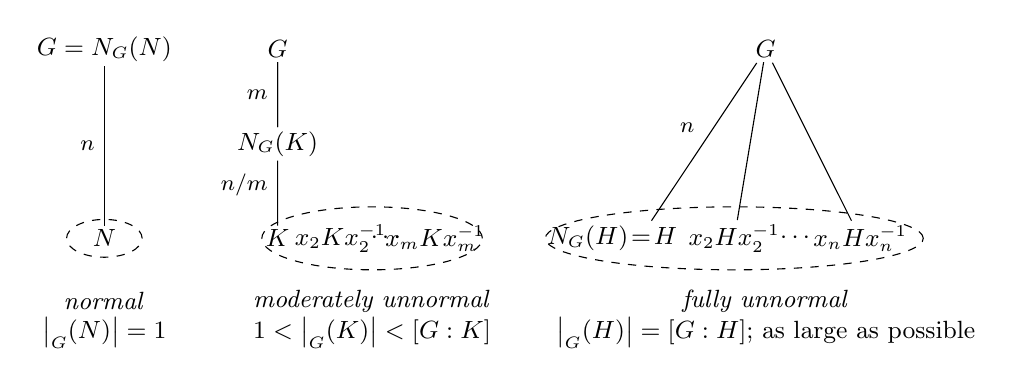
\begin{tikzpicture}[scale=.8]
    \tikzstyle{every node}=[font=\small]
    %%
    \begin{scope}[shift={(0,0)},shorten >= -2pt, shorten <= -2pt]
      \node (G) at (0,3) {$G=\Balert{N_G(N)}$};
      \node (N) at (0,0) {$N$};
      \draw (G)--(N) node[left,pos=.5] {\footnotesize $n$};
      \draw[dashed] (0,0) circle [x radius=.6cm, y radius=.3cm];
      \node at (0,-1) {\Balert{\emph{normal}}};
      \node at (0,-1.5) {$\big|\cl_G(N)\big|=1$};
    \end{scope}
    %%
    \begin{scope}[shift={(4.25,0)},shorten >= -2pt, shorten <= -2pt]
      \node (G) at (-1.5,3) {$G$};
      \node (N_G) at (-1.5,1.5) {\Palert{$N_G(K)$}};
      \node (K) at (-1.5,0) {$K$};
      \node (K2) at (-.5,0) {$x_2Kx_2^{-1}$};
      \node (K3) at (.25,0) {$\cdots$};
      \node (Kl) at (1,0) {$x_m Kx_m^{-1}$};
      \draw (G) -- (N_G);
      \draw (N_G) -- (K) node[left,pos=.35] {\footnotesize $n/m$};
      \draw (G)--(N_G) node[left,pos=.5] {\footnotesize $m$};
      \draw[dashed] (0,0) circle [x radius=1.75cm, y radius=.5cm];
      \node at (0,-1) {\Palert{\emph{moderately unnormal}}};
      \node at (0,-1.5) {$1<\big|\cl_G(K)\big|<[G:K]$};
    \end{scope}
    %%
    \begin{scope}[shift={(10.5,0)},shorten >= -2pt, shorten <= -2pt]
      \node (G) at (0,3) {$G$};
      \node (H) at (-2,0) {\hspace{-7mm}$\Alert{N_G(H)}\!=\!H$};
      \node (H2) at (-.5,0) {$x_2Hx_2^{-1}$};
      \node (H3) at (.5,0) {$\cdots$};
      \node (Hl) at (1.5,0) {$x_n Hx_n^{-1}$};
      \draw (G)--(H) node[above left,pos=.5] {\footnotesize $n$};
      \draw (G) -- (H2); \draw (G) -- (Hl);
      \draw[dashed] (-.5,0) circle [x radius=3cm, y radius=.5cm];
      \node at (0,-1) {\Alert{\emph{fully unnormal}}};
      \node at (0,-1.5) {$\big|\cl_G(H)\big|=[G:H]$; as large as possible};
    \end{scope}
  \end{tikzpicture}
  \]

\end{frame}

%%====================================================================

\begin{frame}{Groups acting on subgroups by conjugation}

  Here is an example of $G=D_3$ acting on its subgroups by a homomorphism $\tau: D_3 \to \Perm(S) \cong S_6$. \vspace{-2mm}

  %% Action graph of D_3 acting on its subgroups
  \[
  \begin{tikzpicture}[scale=.8]
    \tikzstyle{n} = [inner sep=1pt] 
    \tikzstyle{p} = [draw,bend left=30,-stealth]
    \tikzstyle{r-thin} = [draw, eRed, bend left=30, -stealth]
    \tikzstyle{b-thin} = [draw, eBlue, bend left=40, -stealth]
    \tikzstyle{every node}=[font=\small]
    %%
    \begin{scope}[shift={(0,5)}]
      \node [n] (0) at (0,0) {$\tau(1)\quad=\quad$};
      \node [n] (e) at (1,0) {$\<1\>$};
      \node [n] (r) at (2,0) {$\<r\>$};
      \node [n] (f) at (3,0) {$\<f\>$};
      \node [n] (rf) at (4,0) {$\<rf\>$};
      \node [n] (r2f) at (5,0) {$\<r^2f\>$};
      \node [n] (D3) at (6,0) {$D_3$};
    \end{scope}
    %%
    \begin{scope}[shift={(0,4)}]
      \node [n] (0) at (0,0) {\color{xRed} $\tau(r)\quad=\quad$};
      \node [n] (e) at (1,0) {\color{xRed} $\<1\>$};
      \node [n] (r) at (2,0) {\color{xRed} $\<r\>$};
      \node [n] (f) at (3,0) {\color{xRed} $\<f\>$};
      \node [n] (rf) at (4,0) {\color{xRed} $\<rf\>$};
      \node [n] (r2f) at (5,0) {\color{xRed} $\<r^2f\>$};
      \node [n] (D3) at (6,0) {$D_3$};
      \path [r-thin] (f) to (rf);
      \path [r-thin] (rf) to (r2f);
      \path [r-thin] (r2f) to (f);
    \end{scope}
    %%
    \begin{scope}[shift={(0,3)}]
      \node [n] (0) at (0,0) {$\tau(r^2)\quad=\quad$};
      \node [n] (e) at (1,0) {$\<1\>$};
      \node [n] (r) at (2,0) {$\<r\>$};
      \node [n] (f) at (3,0) {$\<f\>$};
      \node [n] (rf) at (4,0) {$\<rf\>$};
      \node [n] (r2f) at (5,0) {$\<r^2f\>$};
      \node [n] (D3) at (6,0) {$D_3$};
      \path [p] (rf) to (f);
      \path [p] (r2f) to (rf);
      \path [p] (f) to (r2f);
    \end{scope}
    %%
    \begin{scope}[shift={(0,2)}]
      \node [n] (0) at (0,0) {\color{xBlue} $\tau(f)\quad=\quad$};
      \node [n] (e) at (1,0) {\color{xBlue} $\<1\>$};
      \node [n] (r) at (2,0) {\color{xBlue} $\<r\>$};
      \node [n] (f) at (3,0) {\color{xBlue} $\<f\>$};
      \node [n] (rf) at (4,0) {\color{xBlue} $\<rf\>$};
      \node [n] (r2f) at (5,0) {\color{xBlue} $\<r^2f\>$};
      \node [n] (D3) at (6,0) {$D_3$};
      \path [b-thin] (rf) to (r2f);
      \path [b-thin] (r2f) to (rf);
    \end{scope}
    %%
    \begin{scope}[shift={(0,1)}]
      \node [n] (0) at (0,0) {$\tau(rf)\quad=\quad$};
      \node [n] (e) at (1,0) {$\<1\>$};
      \node [n] (r) at (2,0) {$\<r\>$};
      \node [n] (f) at (3,0) {$\<f\>$};
      \node [n] (rf) at (4,0) {$\<rf\>$};
      \node [n] (r2f) at (5,0) {$\<r^2f\>$};
      \node [n] (D3) at (6,0) {$D_3$};
      \path [p] (f) to (r2f);
      \path [p] (r2f) to (f);  
    \end{scope}
    %%
    \begin{scope}[shift={(0,0)}]
      \node [n] (0) at (0,0) {$\tau(r^2f)\quad=\quad$};
      \node [n] (e) at (1,0) {$\<1\>$};
      \node [n] (r) at (2,0) {$\<r\>$};
      \node [n] (f) at (3,0) {$\<f\>$};
      \node [n] (rf) at (4,0) {$\<rf\>$};
      \node [n] (r2f) at (5,0) {$\<r^2f\>$};
      \node [n] (D3) at (6,0) {$D_3$};
      \path [p] (f) to (rf);
      \path [p] (rf) to (f);
    \end{scope}
    %%
    \begin{scope}[shift={(9.5,-1.75)},shorten >= -3pt, shorten <= -3pt,
        yscale=1.1]
      \tikzstyle{every node}=[font=\small]
      %%
      \node(G) at (0,6) {$D_3$};
      \node(r) at (-1.75,4.5) {$\<r\>$};
      \node(1) at (0,1.5) {$\<1\>$};
      \node(f) at (.25,24/7) {$\<f\>$};
      \node(rf) at (1.75,24/7) {$\<rf\>$};
      \node(r2f) at (3.25,24/7) {$\<r^2\!f\>$};
      \draw[faded] (G)--(r); 
      \draw[faded] (G)--(f); 
      \draw[faded] (G)--(rf); 
      \draw[faded] (G)--(r2f); 
      \draw[faded] (r)--(1); 
      \draw[faded] (f)--(1);  
      \draw[faded] (rf)--(1); 
      \draw[faded] (r2f)--(1); 
      \draw [r] (f) to (rf);
      \draw [r] (rf) to (r2f);
      \draw [r] (r2f) to [bend left] (f);
      \draw [bb] (rf) to [bend left] (r2f);
      \path (G) edge [r,loop left,>=stealth] (G);
      \path (G) edge [b,loop right,>=stealth] (G);
      \path (r) edge [r,loop left,>=stealth] (r);
      \path (r) edge [b,loop right,>=stealth] (r);
      \path (1) edge [r,loop left,>=stealth] (1);
      \path (1) edge [b,loop right,>=stealth] (1);
      \path (f) edge [b,loop above,>=stealth] (f);
    \end{scope}
  \end{tikzpicture}
  \]
  
  \vspace{-2mm}
  
  \begin{exampleblock}{Observations}
    Do you see how to read stabilizers and fixed points off of the
    permutation diagram? \Pause
    \begin{itemize}
    \item \Balert{$\Ker(\phi)=\<1\>$} consists of the \Balert{row(s)}
      with only fixed points. \Pause
    \item \Galert{$\Fix(\phi)=\big\{\<1\>,\<r\>,D_3\big\}$} consists of the
      \Galert{column(s)} with only fixed points. \Pause
    \item By the orbit-counting theorem, there are
      $|\Alert{\Orb(\phi)}|=24/|D_3|=4$ conjugacy classes.
    \end{itemize}
  \end{exampleblock}
  
\end{frame}

%%====================================================================

\begin{frame}{Groups acting on subgroups by conjugation}

  Here is an example of
  $G=A_4=\<{\color{xRed}(123)},{\color{xBlue}(12)(34)}\>$ acting on its
  subgroups.

  %% Action graph of A_4 acting on its subgroups by conjugation
  \[
  \begin{tikzpicture}[shorten >= -3pt, shorten <= -3pt,auto]
    \tikzstyle{every node}=[font=\normalsize]
    %%
    \begin{scope}[shift={(0,0)},scale=.9]
      \node(A4) at (0,6) {$A_4$};
      \node(V4) at (2.25,4) {$\big\<(12)(34),(13)(24)\big\>$};
      \node(C34) at (-.75,3) {$\big\<(234)\big\>$};
      \node(C33) at (-2.25,3){$\big\<(134)\big\>$};
      \node(C32) at (-3.75,3){$\big\<(124)\big\>$};
      \node(C31) at (-5.25,3) {$\big\<(123)\big\>$};
      \node(C21) at (.75,2) {$\big\<(12)(34))\big\>$};
      \node(C22) at (2.75,2) {$\big\<(13)(24)\big\>$};
      \node(C23) at (4.75,2) {$\big\<(14)(23))\big\>$};
      \node(1) at (0,0) {$\<e\>$};
      \draw[faded] (A4)--(V4);
      \draw[faded] (A4)--(C31);
      \draw[faded] (A4)--(C32);
      \draw[faded] (A4)--(C33);
      \draw[faded] (A4)--(C34);
      \draw[faded] (C31)--(1);
      \draw[faded] (C32)--(1);
      \draw[faded] (C33)--(1);
      \draw[faded] (C34)--(1);
      \draw[faded] (V4)--(C21);
      \draw[faded] (V4)--(C22);
      \draw[faded] (V4)--(C23);
      \draw[faded] (C21)--(1);
      \draw[faded] (C22)--(1);
      \draw[faded] (C23)--(1);
      \path (A4) edge [r,loop left,>=stealth] (A4);
      \path (A4) edge [b,loop right,>=stealth] (A4);
      \path (V4) edge [r,loop above,>=stealth] (V4);
      \path (V4) edge [b,loop below,>=stealth] (V4);
      \path (C31) edge [r,loop above,>=stealth] (C31); 
      \draw [r] (C33) to[bend right=40] (C32);
      \draw [r] (C34) to[bend right=40] (C33);
      \draw [r] (C32) to[bend right=30] (C34);      
      \draw [bb] (C31) to (C32);
      \draw [bb] (C33) to (C34);
      \path (C21) edge [b,loop above,>=stealth] (C21);
      \path (C22) edge [b,loop above,>=stealth] (C22);
      \path (C23) edge [b,loop above,>=stealth] (C23);
      \path (1) edge [r,loop left,>=stealth] (1);
      \path (1) edge [b,loop right,>=stealth] (1);
      \draw [r] (C22) to[bend right=35] (C21);
      \draw [r] (C23) to[bend right=35] (C22);
      \draw [r] (C21) to[bend right=25] (C23);
    \end{scope}
  \end{tikzpicture}
  \]
  
  Let's take a moment to revisit our ``\emph{three favorite examples}''
  from Chapter 3.
  \[
  N=\big\<(12)(34),(13)(24)\big\>,\qquad H=\big\<(123)\big\>,\qquad K
  =\big\<(12)(34)\big\>.
  \]
  
\end{frame}

%%====================================================================

\begin{frame}{Groups acting on subgroups by conjugation}
  
  Here is the ``\emph{fixed point table}'' of the action of $A_4$ on
  its subgroups.
  \[
  \hspace{-5mm}
  \scalebox{.77}{
    \begin{tikzpicture}
      \node at (0,0) {
        \renewcommand\arraystretch{1.7}
        \begin{tabular}{c|cccccccccc}
          & {\small$\<e\>$} & {\small$\<(123)\>$} & {\small$\<(124)\>$} & {\small$\<(134)\>$} & {\small$\<(234)\>$} & {\small$\<(12)(34)\>$} & {\small$\<(13)(24)\>$} & {\small$\<(14)(23)\>$} & {\small$\<(12)(34),(13)(24)\>$} & {\small $A_4$} \\ \hline
          \small $e$ & \checkmark & \checkmark & \checkmark & \checkmark & \checkmark & \checkmark & \checkmark & \checkmark & \checkmark & \checkmark \\
\small $(123)$ & \checkmark & \checkmark & & & & & & & \checkmark & \checkmark \\
\small $(132)$ & \checkmark & \checkmark & & & & & & & \checkmark & \checkmark \\
\small $(124)$ & \checkmark & & \checkmark & & & & & & \checkmark & \checkmark \\
\small $(142)$ & \checkmark & & \checkmark & & & & & & \checkmark & \checkmark \\
\small $(134)$ & \checkmark & & & \checkmark & & & & & \checkmark & \checkmark \\
\small $(143)$ & \checkmark & & & \checkmark & & & & & \checkmark & \checkmark \\
\small $(234)$ & \checkmark & & & & \checkmark & & & & \checkmark & \checkmark \\
\small $(243)$ & \checkmark & & & & \checkmark & & & & \checkmark & \checkmark \\
\small $(12)(34)$ & \checkmark & & & & & \checkmark & \checkmark & \checkmark & \checkmark & \checkmark \\
\small $(13)(24)$ & \checkmark & & & & & \checkmark & \checkmark & \checkmark & \checkmark & \checkmark \\
\small $(14)(23)$ & \checkmark & & & & & \checkmark & \checkmark & \checkmark & \checkmark & \checkmark \\
      \end{tabular}};
  \end{tikzpicture}}
  \]
  
  \Pause
  
  By the \textbf{orbit-counting theorem}, there are 
  $|\Orb(\phi)|=60/|A_4|=5$ conjugacy classes. 
  
\end{frame}

%%====================================================================

\begin{frame}{A summary}
  
  Thus far, we have seen four important (right) actions of a group $G$, acting:

  \begin{itemize}
  \item on itself by multiplication
  \item on itself by conjugation. 
  \item on its subgroups by conjugation. 
  \item on the cosets of a fixed subgroup $H\leq G$ by
    multiplication.
  \end{itemize}
  
  \bigskip  
  \scalebox{.95}{  
    \def\arraystretch{1.75}
    \begin{tabular}{|c|cccc|} \hline
      set $S=$ & \multicolumn{2}{c}{$G$} & subgroups of $G$ & right cosets of $H$ \\ \hline
      operation & multiplication & conjugation  & conjugation &  right multiplication \\ \hline
      $\orb(s)$ & $G$ & $\cl_G(g)$ & $\cl_G(H)$ & all right cosets \\
      $\stab(s)$ & $\<1\>$ & $C_G(g)$ & $N_G(H)$ & $x^{-1}Hx$ \\
      $\fix(g)$ & $G$ or $\emptyset$ & $C_G(g)$ & $\{H\mid g\in N_G(H)\}$ & $\big\{Hx\mid xgx^{-1}\in H\big\}$ \\
      $\Ker(\phi)$ & $\<1\>$ & $Z(G)$ & $\displaystyle\bigcap_{H\leq G} N_G(H)$ &
      largest norm. subgp. $N\leq H$ \\
      $\Fix(\phi)$ & $\emptyset$ & $Z(G)$ & normal subgroups & none \\ \hline
  \end{tabular}}
  
\end{frame}

%%====================================================================

\section{More applications of group actions!}

%%====================================================================
\section*{Cauchy's theorem}
\begin{frame}{A creative application of a group action}

  \begin{block}{Cauchy's theorem} 
    If $p$ is a prime dividing $|G|$, then $G$ has an element (and
    hence a subgroup) of order $p$.
  \end{block}
  
  \begin{exampleblock}{Proof} \Pause
    Let $P$ be the set of ordered $p$-tuples of
    elements from $G$ whose product is $e$: \vspace{-1mm}
    \[
    (x_1,x_2,\dots,x_p)\in P\quad\mbox{iff}\quad x_1x_2\cdots
    x_p=e\,. \Pause
    \]
    Observe that $|P|=|G|^{p-1}$. (We can choose
    $x_1,\dots,x_{p-1}$ freely; then $x_p$ is forced.)
    
    \pause\medskip 
    
    The group $\Z_p$ acts on $P$ by cyclic shift: \vspace{-2
      mm}
    \[
    \phi\colon\Z_p\longrightarrow\Perm(P),\qquad
    (x_1,x_2,\dots,x_p)\stackrel{\phi(1)}{\longmapsto}
    (x_2,x_3\dots,x_p,x_1)\,. %\Pause
    \]
    \Pause The set $P$ is partitioned into orbits, each of size
    $|\orb(s)|=[\Z_p:\stab(s)]=1$ or $p$.
        
    \pause\medskip
    
    The only way that the orbit of $(x_1,x_2,\dots,x_p)$
    can have size $1$ is if $x_1=\cdots=x_p$.

    \Pause\medskip

    Clearly, $(e,\dots,e)\in P$ is a fixed point.
    
    \Pause\medskip
    
    The $|G|^{p-1}-1$ other elements in $P$ sit in orbits of size $1$
    or $p$.
    
    \pause\medskip
    
    Since $p\nmid |G|^{p-1}-1$, there must be other orbits of size
    $1$. \Pause Thus, some $(x,\dots,x)\in P$, with $x\neq e$ satisfies
    $x^p=e$. $\hfill\Box$
  \end{exampleblock}
  
\end{frame}

%%====================================================================

\begin{frame}{Classification of groups of order 6} %\Pause

  By Cauchy's theorem, every group of order $6$ must have:
  \begin{itemize}
  \item an element $\Alert{a}$ of order $3$
    \item an element $\Balert{b}$ of order $2$.
  \end{itemize}
      
  \medskip\Pause

  Clearly, $G=\<\Alert{a},\Balert{b}\>$, and so
   $G$ must have the following ``partial  Cayley graph'':
  %%
  %% Partial Cayley graph of a group of order 6
  \[
  \begin{tikzpicture}[scale=1.1,auto]
    \tikzstyle{every node}=[font=\footnotesize]
    %%
    \node (b) at (0,0) [v] {$b$};
    \node (e) at (0,1) [v] {$e$};
    \node (ba) at (1,0) [v] {$ba$};
    \node (a) at (1,1) [v] {$a$};
    \node (ba2) at (2,0) [v] {$ba^2$};
    \node (a2) at (2,1) [v] {$a^2$};
    \draw [r] (e) to (a); \draw [r] (a) to (a2);
    \draw [r] (a2) to [bend right] (e);
    \draw [r] (b) to (ba); \draw [r] (ba) to (ba2);
    \draw [r] (ba2) to [bend left] (b);
    \draw [bb] (e) to (b);
  \end{tikzpicture}
  \]
  \Pause It is now easy to see that up to isomorphism, there are only $2$
  groups of order $6$: \Pause
  \[
  \begin{tikzpicture}[scale=1.1,auto]
    \tikzstyle{every node}=[font=\footnotesize]
    %%
    \node at (-1.5,.5) {\normalsize $C_6\cong C_2\times C_3$};
    \node (b) at (0,0) [v] {$b$};
    \node (e) at (0,1) [v] {$e$};
    \node (ba) at (1,0) [v] {$ba$};
    \node (a) at (1,1) [v] {$a$};
    \node (ba2) at (2,0) [v] {$ba^2$};
    \node (a2) at (2,1) [v] {$a^2$};
    \draw [r] (e) to (a); \draw [r] (a) to (a2);
    \draw [r] (a2) to [bend right] (e);
    \draw [r] (b) to (ba); \draw [r] (ba) to (ba2);
    \draw [r] (ba2) to [bend left] (b);
    \draw [bb] (e) to (b);
    \draw [bb] (a) to (ba);
    \draw [bb] (a2) to (ba2);      
  \end{tikzpicture}
  \qquad\qquad\qquad\Pause
  \begin{tikzpicture}[scale=1.1,auto]
    \tikzstyle{every node}=[font=\footnotesize]
    \node at (2.75,.5) {\normalsize $D_3$};
    \node (b) at (0,0) [v] {$b$};
    \node (e) at (0,1) [v] {$e$};
    \node (ba) at (1,0) [v] {$ba$};
    \node (a) at (1,1) [v] {$a$};
    \node (ba2) at (2,0) [v] {$ba^2$};
    \node (a2) at (2,1) [v] {$a^2$};
    \draw [r] (e) to (a); \draw [r] (a) to (a2);
    \draw [r] (a2) to [bend right] (e);
    \draw [r] (b) to (ba); \draw [r] (ba) to (ba2);
    \draw [r] (ba2) to [bend left] (b);
    \draw [bb] (e) to (b);
    \draw [bb] (a) to (ba2);
    \draw [bb] (a2) to (ba);      
  \end{tikzpicture}
  \]
  \Pause \textbf{Exercise}. Suppose that $|G| = pq$, where $p < q$ are primes and $p$ doesn't divide $q-1$. Prove that $G$ is cyclic.
  
\end{frame}

%%====================================================================

\section{$p$-groups and the Sylow theorems!}



%%====================================================================

\begin{frame}{$p$-groups and the Sylow theorems} 

  \begin{block}{Definition} 
    A \Alert{$p$-group} is a group whose order is a power of a prime
    $p$. A $p$-group that is a subgroup of a group $G$ is a
    \Alert{$p$-subgroup} of $G$.
  \end{block}

  \Pause\medskip

  Can you tell me some examples of $2$-groups?

  \medskip \Pause

  \begin{exampleblock}{Notational convention}
    Throughout, $G$ will be a group of order $|G|=p^n\cdot m$, with
    $p\nmid m$. 
    
    That is, $p^n$ is the \emph{highest power} of $p$
    dividing $|G|$. (We are isolating all the $p$.)
  \end{exampleblock}

  \medskip\Pause

  There are three \Alert{Sylow theorems}, and loosely speaking, they
  describe the following about a group's $p$-subgroups: \medskip

  \Pause

  \begin{enumerate}
  \item \textbf{Existence}: In every group, $p$-subgroups of all
    possible sizes exist. \Pause\vspace{1mm}
  \item \textbf{Relationship}: All maximal $p$-subgroups are
    conjugate. \Pause\vspace{1mm}
  \item \textbf{Number}: Strong restrictions on the number
    of $p$-subgroups a group can have.
  \end{enumerate}

  \medskip\Pause

  Together, these place strong restrictions on the structure of a
  group $G$ with a fixed order.

\end{frame}

%%====================================================================

\begin{frame}{Groups of order 12 = $2^2 \cdot 3^1$} %\vspace{-10mm}

  \vspace{5mm}

  \begin{columns}
    \begin{column}{.5\textwidth}
      \textbf{Sylow theorems:} \bigskip

      $p$-subgroups come in ``towers.'' \bigskip

      \Balert{2-subgroups blue}; \Alert{3-subgroups red}. \bigskip

      The tops of the towers are conjugate;

      there are restrictions on the size of their conjugacy classes.
    \end{column}
    \begin{column}{.45\textwidth}
    \end{column}
  \end{columns}
  
  
  \vspace{-40mm}

  %% The 5 groups of order 12, with their p-group towers colored
  \[
  \begin{tikzpicture}[scale=.6,auto]
    \newcommand\Hf{6.495} % height of C_12 
    \newcommand\He{5.196} % height of C_6  
    \newcommand\Hd{3.897} % height of C_4 
    \newcommand\Hc{2.598} % height of C_3  
    \newcommand\Hb{1.299} % height of C_2 
    \newcommand\Ha{0} % height of C_1   
    \tikzstyle{every node}=[font=\small]
    %%
    \begin{scope}[shift={(7,7)},scale=1]
      \node(G) at (0,\Hf) {$C_{12}$};
      \draw[cosetBlue,fill=cosetBlue] (1,\Hd)
      circle [x radius=.55cm, y radius=.4cm];
      \draw[cosetRed,fill=cosetRed] (-1,\Hc)
      circle [x radius=.55cm, y radius=.4cm];
      \draw[cosetRed,fill=cosetRed]
      (.55,0)--(-.55,0)--(-1.55,\Hc)--(-.45,\Hc)--(.55,0);
      \draw[cosetBlue,fill=cosetBlue]
      (.55,0)--(-.55,0)--(.45,\Hd)--(1.55,\Hd)--(.55,0);
      \draw[cosetRed,fill=cosetRed,opacity=.6]
      (.55,0)--(-.55,0)--(-1.55,\Hc)--(-.45,\Hc)--(.55,0);
      \draw[cosetPurple,fill=cosetPurple] (0,0)
      circle [x radius=.55cm, y radius=.4cm];
      %%
      \node(C6) at (-.33,\He) {$C_6$};
      \node(C4) at (1,\Hd) {\Balert{$C_4$}};
      \draw[dashed] (1,\Hd) circle [x radius=.5cm, y radius=.35cm];
      \node(C3) at (-1,\Hc) {\Alert{$C_3$}};
      \draw[dashed] (-1,\Hc) circle [x radius=.5cm, y radius=.35cm];
      \node(C2) at (.33,\Hb) {$C_2$};
      \node(C1) at (0,0) {$C_1$};
      %%
      \draw (G) to (C6); \draw (G) to (C4); 
      \draw (C6) to (C3); \draw (C6) to (C2); 
      \draw (C4) to (C2); 
      \draw (C3) to (C1); \draw (C2) to (C1);
    \end{scope}
    %%
    \begin{scope}[shift={(12,7)},scale=1]
      \node(G) at (0,\Hf) {$C_6\times C_2$};
      \draw[cosetBlue,fill=cosetBlue] (1,\Hd)
      circle [x radius=.55cm, y radius=.4cm];
      \draw[cosetRed,fill=cosetRed] (-1,\Hc)
      circle [x radius=.55cm, y radius=.4cm];
      \draw[cosetRed,fill=cosetRed]
      (.55,0)--(-.55,0)--(-1.55,\Hc)--(-.45,\Hc)--(.55,0);
      \draw[cosetBlue,fill=cosetBlue,rounded corners]
      (.55,0)--(-.55,0)--(0,\Hb)--(.45,\Hd)--(1.55,\Hd)--(2.1,\Hb)--(.55,0);
      \draw[cosetRed,fill=cosetRed,opacity=.6]
      (.55,0)--(-.55,0)--(-1.55,\Hc)--(-.45,\Hc)--(.55,0);
      \draw[cosetPurple,fill=cosetPurple]
      (0,0) circle [x radius=.55cm, y radius=.4cm];
      %%
      \node(12) at (-.25,\He) {$C_6$};
      \node(11) at (-1,\He) {$C_6$};
      \node(01) at (-1.75,\He) {$C_6$};
      \node(10-03) at (1,\Hd) {\Balert{$V_4$}};
      \draw[dashed] (1,\Hd) circle [x radius=.5cm, y radius=.35cm];
      \node(02) at (-1,\Hc) {\Alert{$C_3$}};
      \draw[dashed] (-1,\Hc) circle [x radius=.5cm, y radius=.35cm];
      \node(10) at (1.75,\Hb) {$C_2$};
      \node(13) at (1,\Hb) {$C_2$};
      \node(03) at (.25,\Hb) {$C_2$};
      \node(00) at (0,0) {$C_1$};
      %%
      \draw (G) to (12); \draw (G) to (11); 
      \draw (G) to (01);
      \draw (02) to (12); \draw (02) to (11); 
      \draw (02) to (01);
      \draw (10-03) to (G);
      \draw (12) to (10); 
      \draw (11) to (13); 
      \draw (01) to (03);
      \draw (00) to (02);
      \draw (10-03) to (10); \draw (10-03) to (13); 
      \draw (10-03) to (03); 
      \draw (00) to (10); \draw (00) to (13); 
      \draw (00) to (03); 
    \end{scope}
    %%
    \begin{scope}[shift={(-3,0)},scale=1]
      \node(D6) at (0,\Hf) {$D_6$};
      \draw[cosetBlue,fill=cosetBlue] (3,\Hd)
      circle [x radius=1.15cm, y radius=.4cm];
      \draw[cosetRed,fill=cosetRed] (-1.25,\Hc)
      circle [x radius=.55cm, y radius=.4cm];
      \draw[cosetRed,fill=cosetRed]
      (.55,0)--(-.55,0)--(-1.8,\Hc)--(-.7,\Hc)--(.55,0);
      \draw[cosetBlue,fill=cosetBlue,rounded corners]
      (.55,0)--(-.55,0)--(-.25,\Hb)--(1.85,\Hd)--(4.15,\Hd)--(3.9,1.2)--(.55,0);
      \draw[cosetRed,fill=cosetRed,opacity=.6]
      (.55,0)--(-.55,0)--(-1.8,\Hc)--(-.7,\Hc)--(.55,0);
      \draw[cosetPurple,fill=cosetPurple] (0,0)
      circle [x radius=.55cm, y radius=.4cm];
      %%
      \node(r2-f) at (-.25,\He) {$D_3$};
      \node(r2-rf) at (-1,\He) {$D_3$}; 
      \node(r) at (-1.75,\He) {$C_6$}; 
      \node(r3-f) at (2.4,\Hd) {\Balert{$V_4$}};
      \node(r3-rf) at (3,\Hd) {\Balert{$V_4$}};
      \node(r3-r2f) at (3.6,\Hd) {\Balert{$V_4$}};
      %%
      \draw[dashed] (r3-rf) circle [x radius=1.1cm, y radius=.35cm];
      \node(r2) at (-1.25,\Hc) {\Alert{$C_3$}};
      \draw[dashed] (r2) circle [x radius=.5cm, y radius=.35cm];
      %%
      \node(r3) at (0,\Hb) {$C_2$};
      \node(f) at (.6,\Hb) {$C_2$};      
      \node(r4f) at (1.2,\Hb) {$C_2$};
      \node(r2f) at (1.8,\Hb) {$C_2$};
      \node(r3f) at (2.4,\Hb) {$C_2$};
      \node(rf) at (3,\Hb) {$C_2$};
      \node(r5f) at (3.6,\Hb) {$C_2$};
      \node (1) at (0,\Ha) {$C_1$};
      %%
      \draw (D6) -- (r2-f);
      \draw (D6) -- (r);
      \draw (D6) to (r2-rf);
      \draw (D6) to (r3-f); 
      \draw (D6) -- (r3-rf);
      \draw (D6) to (r3-r2f); 
      \draw (r2-rf) to (f); 
      \draw (r2-rf) -- (r2f);
      \draw (r2-rf) to (r4f);
      \draw (r2-f) to (r2);
      \draw (r) -- (r2);
      \draw (r) -- (r3);
      \draw (r2-rf) -- (r2);
      \draw (r2-f) to (rf);
      \draw (r2-f) to (r3f);
      \draw (r2-f) to (r5f);
      \draw (r3-f) -- (f);
      \draw (r3-f) to (r3);
      \draw (r3-f) to (r3f); 
      \draw (r3-rf) to (rf);
      \draw (r3-rf) to (r3);
      \draw (r3-rf) to (r4f); 
      \draw (r3-r2f) to (r2f);
      \draw (r3-r2f) to (r3);
      \draw (r3-r2f) to (r5f);
      \draw (r2) -- (1);
      \draw (f) -- (1);
      \draw (rf) to (1);
      \draw (r2f) to (1);
      \draw (r3f) to (1);
      \draw (r4f) to (1);
      \draw (r5f) to (1); 
      \draw (r3) -- (1);
    \end{scope}
    %%
    \begin{scope}[shift={(4.25,0)},shorten >= -2pt, shorten <= -2pt]
      \node(G) at (0,\Hf) {$\Dic_6$};
      \draw[cosetBlue,fill=cosetBlue] (1,\Hd)
      circle [x radius=1.3cm, y radius=.4cm];
      \draw[cosetRed,fill=cosetRed] (-1.25,\Hc)
      circle [x radius=.55cm, y radius=.45cm];
      \draw[cosetRed,fill=cosetRed]
      (.55,0)--(-.55,0)--(-1.8,\Hc)--(-.7,\Hc)--(.55,0);
      \draw[cosetBlue,fill=cosetBlue,rounded corners]
      (.55,0)--(-.55,0)--(-.4,\Hb)--(-.35,\Hd)--(2.3,\Hd)--(.55,\Hb)--(.55,0);
      \draw[cosetRed,fill=cosetRed,opacity=.6]
      (.55,0)--(-.55,0)--(-1.8,\Hc)--(-.7,\Hc)--(.55,0);
      \draw[cosetPurple,fill=cosetPurple]
      (0,0) circle [x radius=.55cm, y radius=.4cm];
      %%
      \node(b) at (-1,\He) {$C_6$};
      \node(a) at (.25,\Hd) {\Balert{$C_4$}};
      \node(ab) at (1,\Hd) {\Balert{$C_4$}};
      \node(ba) at (1.75,\Hd) {\Balert{$C_4$}};
      \draw[dashed] (1,\Hd) circle [x radius=1.25cm, y radius=.4cm];
      \node(bb) at (-1.25,\Hc) {\Alert{$C_3$}};
      \draw[dashed] (-1.25,\Hc) circle [x radius=.5cm, y radius=.35cm];
      \node(aa) at (0,\Hb) {$C_2$};
      \node(1) at (0,0) {$C_1$};
      \draw (1)--(aa); \draw (1)--(bb);
      \draw(b)--(aa); \draw (b)--(bb);
      \draw(G)--(a); \draw(G)--(ab); \draw(G)--(ba); \draw(G)--(b);
      \draw(aa)--(a); \draw(aa)--(ab); \draw(aa)--(ba);
    \end{scope}
    %%
    \begin{scope}[shift={(10,0)},scale=1]
      \node(A4) at (0,\Hf) {$A_4$};
      \draw[cosetBlue,fill=cosetBlue]
      (1,\Hd) circle [x radius=.55cm, y radius=.4cm];
      \draw[cosetRed,fill=cosetRed]
      (-1.15,\Hc) circle [x radius=1.35cm, y radius=.45cm];
      \draw[cosetRed,fill=cosetRed]
      (.55,0)--(-.55,0)--(-2.5,\Hc)--(.2,\Hc)--(.55,0);
      \draw[cosetBlue,fill=cosetBlue,rounded corners]
      (.55,0)--(-.55,0)--(0,\Hb)--(.45,\Hd)--(1.55,\Hd)--(2.1,1.25)--(.55,0);
      \draw[cosetRed,fill=cosetRed,opacity=.6]
      (.55,0)--(-.55,0)--(-2.5,\Hc)--(.2,\Hc)--(.55,0);
      \draw[cosetPurple,fill=cosetPurple]
      (0,0) circle [x radius=.55cm, y radius=.4cm];
      %%
      \node(V4) at (1,\Hd) {\Balert{$V_4$}};
      \node(C34) at (-.25,\Hc) {\Alert{$C_3$}};
      \node(C33) at (-.85,\Hc){\Alert{$C_3$}};
      \node(C32) at (-1.45,\Hc){\Alert{$C_3$}};
      \node(C31) at (-2.05,\Hc) {\Alert{$C_3$}};
      \node(C21) at (.25,\Hb) {$C_2$};
      \node(C22) at (1,\Hb) {$C_2$};
      \node(C23) at (1.75,\Hb) {$C_2$};
      \node(1) at (0,0) {$C_1$};
      %%
      \draw (A4)--(V4);
      \draw(A4)--(C31);
      \draw(A4)--(C32);
      \draw(A4)--(C33);
      \draw(A4)--(C34);
      \draw(C31)--(1);
      \draw(C32)--(1);
      \draw(C33)--(1);
      \draw(C34)--(1);
      \draw(V4)--(C21);
      \draw(V4)--(C22);
      \draw(V4)--(C23);
      \draw(C21)--(1);
      \draw(C22)--(1);
      \draw(C23)--(1);
      \draw[dashed] (1,\Hd) circle [x radius=.5cm, y radius=.35cm];
      \draw[dashed] (-1.15,\Hc) circle [x radius=1.3cm, y radius=.4cm];
    \end{scope}
  \end{tikzpicture}
  \]
  
\end{frame}

%%====================================================================

\begin{frame}{$p$-groups} %\Pause

  Before we introduce the Sylow theorems, we need to better understand
  $p$-groups.

  \Pause\medskip
  
  \begin{block}{$p$-group Lemma}
    If a $p$-group $G$ acts on a set $S$ via $\phi\colon
    G\to\Perm(S)$, then
    \[
    |\Fix(\phi)|\equiv_p|S|.
    \]
    $\;$\vspace{-5mm}
  \end{block}

  \begin{exampleblock}{Proof (sketch)} \Pause
    \begin{columns}
      \begin{column}{.45\textwidth}
        Suppose $|G|=p^n$. 
        
        \bigskip\Pause 
        
        By the orbit-stabilizer theorem, the only possible orbit sizes
        are $1,p,p^2,\dots,p^n$.
      \end{column}
      
      \begin{column}{.5\textwidth}
        \vspace{-3mm}
        %%
        %% Sketch of the p-group lemma (fixed points & orbits of size p^k)
        \begin{center}
          \tikzstyle{v} = [circle, draw,inner sep=0pt, minimum size=1mm]
          \tikzstyle{r} = [draw, eRed, -stealth]
          %%
          \begin{tikzpicture}[scale=.5, auto]
            \node at (-3,3.5) {\footnotesize $\Fix(\phi)$};
            \node at (3.25,3.5) {\footnotesize
              non-fixed points all in size-$p^k$ orbits};
            \node at (-3.5,-.5) [v] {};
            \node at (-2.5,.5) [v] {};
            \node at (-3.5,1.5) [v] {};
            \node at (-2.5,2.5) [v] {};
            %%
            \begin{scope}[shift={(0,2)}]
              \node (0) at (90:1) [v] {};
              \node (1) at (38.6:1) [v] {};
              \node (2) at (-12.9:1) [v] {};
              \node (3) at (-64.3:1) [v] {};
              \node (4) at (-115.7:1) [v] {};
              \node (5) at (-167.1:1) [v] {};
              \node (6) at (141.4:1) [v] {};
              \path[r] (0) to [bend left=15] (1);
              \path[r] (1) to [bend left=15] (2);
              \path[r] (2) to [bend left=15] (3);
              \path[r] (3) to [bend left=15] (4);
              \path[r] (4) to [bend left=15] (5);
              \path[r] (5) to [bend left=15] (6);
              \path[r] (6) to [bend left=15] (0);
              \node at (0,0) {\footnotesize $p$ elts};
            \end{scope}
            %%
            \begin{scope}[shift={(1.5,0)}]
              \node (0) at (90:1) [v] {};
              \node (1) at (30:1) [v] {};
              \node (2) at (-30:1) [v] {};
              \node (3) at (-90:1) {};
              \node (4) at (-150:1) {};
              \node (5) at (150:1) [v] {};
              \node at (-100:1) {\color{xRed} $\cdot$};
              \node at (-120:1) {\color{xRed} $\cdot$};
              \node at (-140:1) {\color{xRed} $\cdot$};
              \path[r] (0) to [bend left=15] (1);
              \path[r] (1) to [bend left=15] (2);
              \path[r] (2) to [bend left=15] (3);
              \path[r] (4) to [bend left=15] (5);
              \path[r] (5) to [bend left=15] (0);
              \node at (0,0) {\footnotesize $p^3$ elts};
            \end{scope}
            %%
            \begin{scope}[shift={(3,2)}]
              \node (0) at (90:1) [v] {};
              \node (1) at (30:1) [v] {};
              \node (2) at (-30:1) [v] {};
              \node (3) at (-90:1) {};
              \node (4) at (-150:1) {};
              \node (5) at (150:1) [v] {};
              \node at (-100:1) {\color{xRed} $\cdot$};
              \node at (-120:1) {\color{xRed} $\cdot$};
              \node at (-140:1) {\color{xRed} $\cdot$};
              \path[r] (0) to [bend left=15] (1);
              \path[r] (1) to [bend left=15] (2);
              \path[r] (2) to [bend left=15] (3);
              \path[r] (4) to [bend left=15] (5);
              \path[r] (5) to [bend left=15] (0);
              \node at (0,0) {\footnotesize $p^i$ elts};
            \end{scope}
            %%
            \begin{scope}[shift={(4.5,0)}]
              \node (0) at (90:1) [v] {};
              \node (1) at (38.6:1) [v] {};
              \node (2) at (-12.9:1) [v] {};
              \node (3) at (-64.3:1) [v] {};
              \node (4) at (-115.7:1) [v] {};
              \node (5) at (-167.1:1) [v] {};
              \node (6) at (141.4:1) [v] {};
              \path[r] (0) to [bend left=15] (1);
              \path[r] (1) to [bend left=15] (2);
              \path[r] (2) to [bend left=15] (3);
              \path[r] (3) to [bend left=15] (4);
              \path[r] (4) to [bend left=15] (5);
              \path[r] (5) to [bend left=15] (6);
              \path[r] (6) to [bend left=15] (0);
              \node at (0,0) {\footnotesize $p$ elts};
            \end{scope}
            %%
            \begin{scope}[shift={(6,2)}]
              \node (0) at (90:1) [v] {};
              \node (00) at (60:1) [v] {};
              \node (1) at (30:1) [v] {};
              \node (11) at (0:1) [v] {};
              \node (2) at (-30:1) [v] {};
              \node (22) at (-60:1) [v] {};
              \node (3) at (-110:1) {};
              \node (4) at (-150:1) {};
              \node (5) at (150:1) [v] {};
              \node (55) at (120:1) [v] {};
              \node at (-110:1) {\color{xRed} $\cdot$};
              \node at (-130:1) {\color{xRed} $\cdot$};
              \node at (-150:1) {\color{xRed} $\cdot$};
              \path[r] (0) to [bend left=15] (00);
              \path[r] (00) to [bend left=15] (1);
              \path[r] (1) to [bend left=15] (11);
              \path[r] (11) to [bend left=15] (2);
              \path[r] (2) to [bend left=15] (22);
              \path[r] (22) to [bend left=15] (3);
              \path[r] (4) to [bend left=15] (5);
              \path[r] (5) to [bend left=15] (55);
              \path[r] (55) to [bend left=15] (0);
              \node at (0,0) {\footnotesize $p^6$ elts};
            \end{scope}
          \end{tikzpicture}
        \end{center}
      \end{column}
    \end{columns}      
  \end{exampleblock} \Pause

  A lot of proofs about $p$-groups go like this: two things are equal mod $p$; set up some action of $G$ on $S$; one of the things is the number of fixed points; the other thing is the size of $S$.
  
\end{frame}

%%====================================================================

\begin{frame}{$p$-groups} %\medskip

  \begin{block}{Normalizer lemma, Part 1}
    If $H$ is a $p$-subgroup of $G$, then \vspace{-1mm}
    \[
    [N_G(H)\colon H]\equiv_p[G\colon H]\,.
    \]
    $\;$\vspace{-0.4cm}
  \end{block}
  
  \smallskip\Pause
  
  \textbf{Approach}:
  \begin{itemize}
  \item Let $H$ (not $G$!) act on the (right) cosets of $H$ by (right)
    multiplication. \Pause
    \[
    \begin{tikzpicture}[scale=.7]
      \draw[thin,fill=boxBlue] (0,0) rectangle (1,3);
      \draw[thin,fill=boxBlue] (1,0) rectangle (2,3);
      \draw[thin,fill=boxBlue] (3,0) rectangle (4,3);
      \draw[thin,fill=boxRed] (4,0) rectangle (5,3);
      \draw[thin,fill=boxRed] (8,0) rectangle (9,3);
      \draw[thin,fill=boxRed] (5,2) rectangle (8,3);
      \draw[thin,fill=boxRed] (5,1) rectangle (8,2);
      \draw[thin] (0,0) rectangle (9,3);
      \node at (.5,1.5) {\small $H$};
      \node at (1.5,1.5) {\small $Hx_2$};
      \node at (3.5,1.5) {\small $Hx_k$};
      \node at (4.5,1.5) {\small $Hy_1$};
      \node at (6.5,2.5) {\small $Hy_2$};
      \node at (6.5,1.5) {\small $Hy_3$};
      \node at (6.5,0.6) {$\vdots$};
      \node at (2.5,1.5) {\dots};
      \draw[decorate,decoration={brace,amplitude=5pt,mirror}] (0,-.2)--(4,-.2); 
      \node at (2.2,-.8) {\small
        \emph{Cosets of $H$ in $N_G(H)$ are the fixed points}};
      \draw[decorate,decoration={brace,amplitude=5pt}] 
      (0,3.2) --  (9,3.2); 
      \node at (4.5,3.8) {\small \emph{$S$ is the set of cosets of $H$ in $G$}};
    \end{tikzpicture}
    \]
    \Pause
  \item Apply our lemma: $|\Fix(\phi)|\equiv_p|S|$.
  \end{itemize}
  
\end{frame}

%%====================================================================

\begin{frame}{$p$-groups} \medskip

  \begin{block}{Normalizer lemma, Part 1}
    If $H$ is a $p$-subgroup of $G$, then \vspace{-1mm}
    \[
    [N_G(H)\colon H]\equiv_p[G\colon H]\,.
    \]
    $\;$\vspace{-0.4cm}
  \end{block}

  \vspace{-1mm}

  \begin{exampleblock}{Proof}
    Let $S=H\!\setminus\!G=\{Hx\mid x\in G\}$. \Pause The group $H$
    acts on $S$ by \textbf{right-multiplication}, via $\phi\colon
    H\to\Perm(S)$, where
    \[
    \phi(h)=\mbox{\footnotesize the permutation sending each $Hx$ to
      $Hxh$.}
    \]
    
    \pause
    
    The {\color{xGreen}fixed points} of $\phi$ are the cosets $Hx$
    in the {\color{xGreen}normalizer $N_G(H)$}: \Pause\vspace{-2mm}
    \[
    \renewcommand{\arraystretch}{1.2}
    \begin{array}{lll}
      Hxh=Hx,\quad\forall h\in H\quad & \Longleftrightarrow\quad &
      Hxhx^{-1}=H,\quad\forall h\in H\Pause
      \\ & \Longleftrightarrow\quad & xhx^{-1}\in H,\quad\forall h\in H\,
      \Pause \\ & \Longleftrightarrow\quad & x\in N_G(H)\,.
    \end{array}
    \]

    \pause
    
    Therefore, $|\Fix(\phi)|=[N_G(H)\colon H]$, and
    $|S|=[G:H]$. \Pause By our $p$-group Lemma,
    \[
    \quad\qquad\qquad\qquad|\Fix(\phi)|\equiv_p|S|
    \quad\Longrightarrow\quad\Pause {[N_G(H)\colon H]}\equiv_p[G\colon H].
    \qquad\qquad\qquad\quad\Box
    \] \vspace{-4mm}
  \end{exampleblock}
  
\end{frame}

%%====================================================================

\begin{frame}{$p$-groups}
  
  Here is a picture of the action of the $p$-subgroup $H$ (for $p=2$) on the set
  $S=H\!\setminus\!G$, from the proof of the normalizer lemma.
  
  %%
  %% Picture of the orbits in the p-group lemma (from VGT)
  %% Updated picture of the normalizer lemma, and orbits of cosets.
  %%
  \[
  \begin{tikzpicture}[scale=.95]
    \tikzstyle{v-r} = [circle,draw,fill=boxRed,inner sep=0pt,minimum size=4.5mm]
    \tikzstyle{v-b} = [circle,draw,fill=boxBlue,inner sep=0pt,
      minimum size=4.5mm]
    \tikzset{every loop/.style={min distance=4mm,looseness=8}}
    %%
    \begin{scope}[shift={(0,0)}]
      \node at (-.5,2.5) {$\bm{\Fix(\phi)}$};
      \draw[decorate,decoration={brace,amplitude=5pt,mirror}] 
      (-2.25,-3.2) --  (1.25,-3.2); 
      \node at (-.25,-3.7) {\small\it The fixed points are the};
      \node at (-.25,-4.1) {\small\it cosets in $N_G(H)$};
      \draw[decorate,decoration={brace,amplitude=5pt,mirror}] 
      (1.75,-3.2) --  (8.5,-3.2); 
      \node at (5,-3.7) {\small\it Cosets not in $N_G(H)$ are in orbits};
      \node at (5,-4.1) {\small\it of order $p^i$, for various $i\geq 1$};
      \node (1) at (-1,1) [v-b] {\small $H$};
      \node (a1) at (0,0) [v-b] {\small $Ha_1$};
      \node (a2) at (-1,-1) [v-b] {\small $Ha_2$};
      \node (a3) at (0,-2) [v-b] {\small $Ha_3$};
      %%
      \path (1) edge [r,loop left,>=stealth] (1);
      \path (1) edge [b,loop right,>=stealth] (1);
      \path (a1) edge [r,loop left,>=stealth] (a1);
      \path (a1) edge [b,loop right,>=stealth] (a1);
      \path (a2) edge [r,loop left,>=stealth] (a2);
      \path (a2) edge [b,loop right,>=stealth] (a2);
      \path (a3) edge [r,loop left,>=stealth] (a3);
      \path (a3) edge [b,loop right,>=stealth] (a3);
    \end{scope}
    %%
    \begin{scope}[shift={(2.75,2.2)}]
      \tikzstyle{every node}=[font=\footnotesize]
      \tikzstyle{to} = [draw,thick]
      %%
      \node (g1) at (0,0) [v-r] {$Hb_1$};
      \node (g2) at (1.5,0) [v-r] {$Hb_2$};
      \draw[rr] (g1) to [bend left=10] (g2);
      \draw[bb] (g1) to[bend right=10] (g2);
    \end{scope}
    %%
    \begin{scope}[shift={(2.75,1.2)}]
      \tikzstyle{every node}=[font=\footnotesize]
      \tikzstyle{to} = [draw,thick]
      %%
      \node (g1) at (0,0) [v-r] {$Hg_1$};
      \node (g2) at (1.5,0) [v-r] {$Hg_2$};
      \draw[rr] (g1) -- (g2);
      \path (g1) edge [b,loop left,>=stealth] (g1);
      \path (g2) edge [b,loop right,>=stealth] (g2);
    \end{scope}
    %%
    \begin{scope}[shift={(3.5,-1.2)}]
      \tikzstyle{every node}=[font=\footnotesize]
      \tikzstyle{to} = [draw, Red,-stealth,bend right=9,very thick]
      %%
      \node (g7) at (0:1.35) [v-r] {$Hg_7$};
      \node (g8) at (45:1.35) [v-r] {$Hg_8$};
      \node (g9) at (90:1.35) [v-r] {$Hg_9$};
      \node (g10) at (135:1.35) [v-r] {\scriptsize $Hg_{10}$};
      \node (g11) at (180:1.35) [v-r] {\scriptsize $Hg_{11}$};
      \node (g12) at (225:1.35) [v-r] {\scriptsize $Hg_{12}$};
      \node (g13) at (270:1.35) [v-r] {\scriptsize $Hg_{13}$};
      \node (g14) at (315:1.35) [v-r] {\scriptsize $Hg_{14}$};
      \draw [r] (g7) to (g8);
      \draw [r] (g8) to (g9);
      \draw [r] (g9) to (g10);
      \draw [r] (g10) to (g11);
      \draw [r] (g11) to (g12);
      \draw [r] (g12) to (g13);
      \draw [r] (g13) to (g14);
      \draw [r] (g14) to (g7);
      \draw [bb] (g7) to (g9);
      \draw [bb] (g10) to (g14);
      \draw [bb] (g11) to (g13);
      \path (g8) edge [b,in=30, out=60,loop,>=stealth] (g8); 
      \path (g12) edge [b,in=210, out=240,loop,>=stealth] (g12);
    \end{scope}
    %%
    \begin{scope}[shift={(7,1.5)}]
      \tikzstyle{every node}=[font=\footnotesize]
      \tikzstyle{r} = [draw, eRed, -stealth,bend right=20,very thick]
      %%
      \node (g3) at (0:.9) [v-r] {$Hc_1$};
      \node (g4) at (90:.9) [v-r] {$Hc_2$};
      \node (g5) at (180:.9) [v-r] {$Hc_3$};
      \node (g6) at (270:.9) [v-r] {$Hc_4$};
      \draw [r] (g3) to (g4);
      \draw [r] (g4) to (g5);
      \draw [r] (g5) to (g6);
      \draw [r] (g6) to (g3);
      \draw [bb] (g4) to (g6);
      \path (g5) edge [b,loop left,>=stealth] (g5);
      \path (g3) edge [b,loop right,>=stealth] (g3);
    \end{scope}
    %%
    \begin{scope}[shift={(7,-1.5)}]
      \tikzstyle{every node}=[font=\footnotesize]
      \tikzstyle{r} = [draw, eRed, -stealth,bend right=20,very thick]
      %%
      \node (g3) at (0:.9) [v-r] {$Hg_3$};
      \node (g4) at (90:.9) [v-r] {$Hg_4$};
      \node (g5) at (180:.9) [v-r] {$Hg_5$};
      \node (g6) at (270:.9) [v-r] {$Hg_6$};
      \draw [r] (g3) to (g4);
      \draw [r] (g4) to (g5);
      \draw [r] (g5) to (g6);
      \draw [r] (g6) to (g3);
      \draw [bb] (g3) to (g4); \draw [bb] (g5) to (g6);
    \end{scope}
  \end{tikzpicture}
  \]
  
\end{frame}

%%====================================================================

\begin{frame}{$p$-subgroups} %\Pause
  
  Recall that $H\leq N_G(H)$ (always), and $H$ is \Alert{fully
    unnormal} if $H=N_G(H)$. 
  
  \smallskip\Pause
  
  \begin{block}{Normalizer lemma, Part 2} 
    Suppose $|G|=p^nm$, and $H\leq G$ with $|H|=p^i<p^n$. Then $H\lneq
    N_G(H)$, and the index $[N_G(H):H]$ is a multiple of $p$. \Pause
  \end{block}
  
  %% The red/blue coset partition, illustrating the normalizer lemma, Part 2
  \[
  \begin{tikzpicture}[scale=.7]
    \draw[thin,fill=boxBlue] (0,0) rectangle (1,3);
    \draw[thin,fill=boxBlue] (1,0) rectangle (2,3);
    \draw[thin,fill=boxBlue] (3,0) rectangle (4,3);
    \draw[thin,fill=boxRed] (4,0) rectangle (5,3);
    \draw[thin,fill=boxRed] (8,0) rectangle (9,3);
    \draw[thin,fill=boxRed] (5,2) rectangle (8,3);
    \draw[thin,fill=boxRed] (5,1) rectangle (8,2);
    \draw[thin] (0,0) rectangle (9,3);
    \node at (.5,1.5) {\small $H$};
    \node at (1.5,1.5) {\small $Hx_2$};
    \node at (3.5,1.5) {\small $Hx_k$};
    \node at (4.5,1.5) {\small $Hy_1$};
    \node at (6.5,2.5) {\small $Hy_2$};
    \node at (6.5,1.5) {\small $Hy_3$};
    \node at (6.5,0.6) {$\vdots$};
    \node at (2.5,1.5) {\dots};
    \draw[decorate,decoration={brace,amplitude=5pt,mirror}] (0,-.2)--(4,-.2); 
    \node at (2.2,-.8) {\small
      $[N_G(H):H]>1$ cosets of $H$ (a multiple of $p$)};
    \draw[decorate,decoration={brace,amplitude=5pt}] (0,3.2) -- (9,3.2); 
    \node at (4.5,3.8) {\small $[G:H]$ cosets of $H$ (a multiple of $p$)};
    \node at (-3,1.9) {$H$ is not ``\emph{fully unnormal}'':};
    \node at (-3,1.1) {$H\lneq N_G(H)\leq G$};
  \end{tikzpicture}
  \]
  
  \Pause\vspace{-3mm}
  
  \begin{alertblock}{Important corollaries}
    \begin{itemize}
    \item $p$-groups cannot have any fully unnormal subgroups (i.e.,
      $H\lneq N_G(H)$).
    \item In \emph{any} finite group, the only fully unnormal $p$-subgroups
      are maximal.
    \end{itemize}  
  \end{alertblock}
  
\end{frame}

%%====================================================================

\begin{frame}{Normalizers of $p$-subgroups}

  Let $H$ be properly contained in a maximal $p$-subgroup $P\lneq G$. \smallskip
  
  \begin{itemize}
  \item The normalizer of $H$ \emph{must} grow in $P$ (and hence in $G$)
    \smallskip
  \item The normalizer of $P$ \emph{need not} grow in $G$. 
  \end{itemize}
  
  %% Red/blue coset partition illustrating the normalizers of p-groups
  \[
  \begin{tikzpicture}[scale=.5]
    \begin{scope}[shift={(0,0)}]
      \begin{scope}[shift={(0,0)}]
        \tikzstyle{every node}=[font=\footnotesize]
        %%
        \draw[color=boxBlue,fill=boxBlue] (0,0) rectangle (1,3);
        \draw[color=boxBlue,fill=boxBlue] (1,0) rectangle (2,3);
        \draw[color=boxRed,fill=boxRed] (2,2) rectangle (5,3);
        \draw[color=boxRed,fill=boxRed] (2,1) rectangle (5,2);
        \draw[very thin] (1,0) to (1,3); \draw[very thin] (2,0) to (2,3);
        \draw[very thin] (2,1) to (5,1); \draw[very thin] (2,2) to (5,2);
        \draw[ultra thick] (0,0) rectangle (5,3);
        \node at (.5,1.5) {$H$};
        \node at (1.5,1.5) {$Ha$};
        \node at (4,2.5) {$Hb$};
        \node at (4,1.5) {$Hc$};
        \node at (4,0.65) {$\vdots$};
        \node at (2.75,1.5) {\large\bf $\mathbf{P}$};
        \node at (2.5,4.2) {\small $H\lneq N_P(H)\leq N_G(H)$};
        \draw[decorate,decoration={brace,amplitude=5pt}] (0,3.2) --  (2,3.2); 
      \end{scope}
      %%
      \begin{scope}[shift={(5,0)}]
        \draw (0,0) rectangle (1,3);
        \draw (1,0) rectangle (2,3);
        \draw (2,2) rectangle (5,3);
        \draw (2,1) rectangle (5,2);
        \draw[very thin] (1,0) to (1,3); \draw[very thin] (2,0) to (2,3);
        \draw[very thin] (2,1) to (5,1); \draw[very thin] (2,2) to (5,2);
        \draw[ultra thick] (0,0) rectangle (5,3);
        \node at (.5,1.5) {};
        \node at (1.5,1.5) {};
        \node at (3.5,2.5) {};
        \node at (3.5,1.5) {};
        \node at (3.5,0.6) {};
        \filldraw[fill=white,opacity=0.7] (0,0)--(0,3)--(5,3)--(5,0)--cycle;
        \node at (2.75,1.5) {\large\bf $\mathbf{xP}$};
      \end{scope}
      %%
      \begin{scope}[shift={(0,-3)}]
        \draw (0,0) rectangle (1,3);
        \draw (1,0) rectangle (2,3);
        \draw (2,2) rectangle (5,3);
        \draw (2,1) rectangle (5,2);
        \draw[very thin] (1,0) to (1,3); \draw[very thin] (2,0) to (2,3);
        \draw[very thin] (2,1) to (5,1); \draw[very thin] (2,2) to (5,2);
        \draw[ultra thick] (0,0) rectangle (5,3);
        \node at (.5,1.5) {};
        \node at (1.5,1.5) {};
        \node at (3.5,2.5) {};
        \node at (3.5,1.5) {};
        \node at (3.5,0.6) {};
        \filldraw[fill=white,opacity=0.7] (0,0)--(0,3)--(5,3)--(5,0)--cycle;
        \node at (2.75,1.5) {\large\bf $\mathbf{yP}$};
      \end{scope}
      %%
      \begin{scope}[shift={(5,-3)}]
        \draw (0,0) rectangle (1,3);
        \draw (1,0) rectangle (2,3);
        \draw (2,2) rectangle (5,3);
        \draw (2,1) rectangle (5,2);
        \draw[very thin] (1,0) to (1,3); \draw[very thin] (2,0) to (2,3);
        \draw[very thin] (2,1) to (5,1); \draw[very thin] (2,2) to (5,2);
        \draw[ultra thick] (0,0) rectangle (5,3);
        \node at (.5,1.5) {};
        \node at (1.5,1.5) {};
        \node at (3.5,2.5) {};
        \node at (3.5,1.5) {};
        \node at (3.5,0.6) {};
        \filldraw[fill=white,opacity=0.7] (0,0)--(0,3)--(5,3)--(5,0)--cycle;
        \node at (2.75,1.5) {\large\bf $\mathbf{zP}$};
      \end{scope}
    \end{scope}
    %%%%%%%%%%%%%%%%%%%%%%%%%%%%%%%%%%%%%%%%%%%%%%%%%%%%%%%%
    \begin{scope}[shift={(12.5,0)}]
      \begin{scope}[shift={(0,0)}]
        \tikzstyle{every node}=[font=\footnotesize]
        %%
        \draw[color=boxBlue,fill=boxBlue] (0,0) rectangle (5,3);
        \draw[ultra thick] (0,0) rectangle (5,3);
        \node at (2.75,1.5) {\large\bf $\mathbf{P}$};
        \node at (4,4.2) {\small \emph{it may happen that $P=N_G(P)$}};
        \draw[decorate,decoration={brace,amplitude=5pt}] (0,3.2) --  (5,3.2); 
      \end{scope}
      %%
      \begin{scope}[shift={(5,0)}]
        \draw[color=boxRed,fill=boxRed] (0,0) rectangle (5,3);
        \draw[ultra thick] (0,0) rectangle (5,3);
        \node at (2.75,1.5) {\large\bf $\mathbf{xP}$};
      \end{scope}
      %%
      \begin{scope}[shift={(0,-3)}]
        \draw[color=boxRed,fill=boxRed] (0,0) rectangle (5,3);
        \draw[ultra thick] (0,0) rectangle (5,3);
        \node at (2.75,1.5) {\large\bf $\mathbf{yP}$};
      \end{scope}
      %%
      \begin{scope}[shift={(5,-3)}]
        \draw[color=boxRed,fill=boxRed] (0,0) rectangle (5,3);
        \draw[ultra thick] (0,0) rectangle (5,3);
        \node at (2.75,1.5) {\large\bf $\mathbf{zP}$};
      \end{scope}
    \end{scope}
  \end{tikzpicture}
  \]
  
\end{frame}

%%====================================================================

\begin{frame}{Proof of the normalizer lemma}

  \begin{block}{Normalizer lemma, Part 2} 
    Suppose $|G|=p^nm$, and $H\leq G$ with $|H|=p^i<p^n$. Then $H\lneq
    N_G(H)$, and the index $[N_G(H):H]$ is a multiple of $p$. 
  \end{block}

  \begin{exampleblock}{Proof} 
    Since $H\normaleq N_G(H)$, we can create the quotient map 
    \[
    \pi\colon N_G(H)\longrightarrow N_G(H)/H\,,\qquad\qquad \pi\colon
    g\longmapsto gH\,. \Pause
    \]
    The size of the quotient group is $[N_G(H)\colon H]$, the number of
    cosets of $H$ in $N_G(H)$.
    
    \pause\bigskip
    
    By the normalizer lemma Part 1, $[N_G(H)\colon H]\equiv_p[G\colon
      H]$. \Pause By Lagrange's theorem, %\Pause
    \[
    [N_G(H)\colon H]\equiv_p[G\colon
      H]=\frac{|G|}{|H|}\Pause=\frac{p^nm}{p^i}=p^{n-i}m\equiv_p 0.
    \]
    \pause Therefore, $[N_G(H)\colon H]$ is a multiple of $p$, so $N_G(H)$
    must be strictly larger than $H$. $\hfill\Box$
  \end{exampleblock}
  
\end{frame}

%%====================================================================

\begin{frame}{The Sylow theorems} %\Pause

  Recall the following question that we asked earlier in this
  course. \smallskip
  
  \begin{exampleblock}{Open-ended question}
    What group structural properties are possible, what are
    impossible, and how does this depend on $|G|$?
  \end{exampleblock}

  \smallskip\Pause
  
  One approach is to decompose large groups into ``building block
  subgroups.'' \Pause For example:
  
  \smallskip
  
  \begin{quote}
    \emph{given a group of order $72=2^3\cdot 3^2$, what can we say
      about its $2$-subgroups and $3$-subgroups?}.
  \end{quote}
    
  \smallskip\Pause

  This is the idea behind the \Alert{Sylow theorems}, developed by
  Norwegian mathematician Peter Sylow (1832--1918). \medskip\Pause

  The Sylow theorems address the following questions of a finite group $G$:
  
  \smallskip\Pause
  
  \begin{enumerate}
    \item How big are its $p$-subgroups? \smallskip\Pause
    \item How are the $p$-subgroups related? \smallskip\Pause
    \item How many $p$-subgroups are there? \smallskip\Pause
    \item Are any of them normal? 
  \end{enumerate}
  
\end{frame}

%%====================================================================

\begin{frame}{The Sylow theorems}

  \begin{alertblock}{Notational convention}
    Througout, $G$ will be a group of order $|G|=p^n\cdot m$, with
    $p\nmid m$. \medskip\Pause

    That is, $p^n$ is the \emph{highest power} of $p$ dividing
    $|G|$. \medskip\Pause

    A subgroup of order $p^n$ is called a \Alert{Sylow
      $p$-subgroup}. \medskip\Pause
    
    Let $\Syl_p(G)$ denote the set of Sylow $p$-subgroups, and
    \Balert{$n_p:=\big|\Syl_p(G)\big|$}.
  \end{alertblock}

  \medskip\Pause

  There are three \Alert{Sylow theorems}, and loosely speaking, they
  describe the following about a group's $p$-subgroups:

  \smallskip\Pause

  \begin{enumerate}
  \item \textbf{Existence}: In every group, $p$-subgroups of all
    possible sizes exist, and they're ``\emph{nested}''. \smallskip\Pause
  \item \textbf{Relationship}: All maximal $p$-subgroups are
    conjugate. \smallskip\Pause
  \item \textbf{Number}: There are strong restrictions on $n_p$, the
    number of Sylow $p$-subgroups.
  \end{enumerate}

  \medskip\Pause

  Together, these place strong restrictions on the structure of a
  group $G$ with a fixed order.  

\end{frame}

%%====================================================================

\begin{frame}{Our unknown group of order 12} %\Pause

  Throughout, we will have a running example, a ``mystery group'' $G$
  of order $12=2^2\cdot 3$. \medskip\Pause

  We already know a little bit about $G$. By \Balert{Cauchy's
    theorem}, it must have: \smallskip
  \begin{itemize}
  \item an element $a$ of order $2$, and \smallskip\Pause
  \item an element $b$ of order $3$.
  \end{itemize}
  
  \vspace{-8mm}
  
  %% Our unknown group of order 12: using Cauchy's theorem only
  \[
  \begin{tikzpicture}[scale=.6]
    \newcommand\Hf{6.495} % height of C_12 
    \newcommand\He{5.196} % height of C_6  
    \newcommand\Hd{3.897} % height of C_4 
    \newcommand\Hc{2.598} % height of C_3  
    \newcommand\Hb{1.299} % height of C_2 
    \newcommand\Ha{0} % height of C_1   
    %%
    \begin{scope}[scale=1.45,shift={(0,3.15)}]
      \node at (1.2,1) {\small $|G|\!=\!12$};
      \draw [midgray,very thick] (-1.5,-3.3) rectangle (2,1.4);
      \draw [eRed,very thick] (0,.02)
      circle [y radius=1.25cm, x radius=.5cm,rotate=-10];
      \draw [eBlue,very thick] (-.62,-.94)
      circle [x radius=.4cm, y radius=.65cm,rotate=90];
      \node at (-.1,-.96) {\color{xPurple}\footnotesize $e$};
      \node at (-.3,-.94) {\color{xPurple}$\bullet$};
      \node at (-.1,.25) {\color{xRed}\footnotesize $b$};
      \node at (-.1,0) {$\color{xRed}\bullet$};
      \node at (.15,.95) {\color{xRed}\footnotesize $b^2$};
      \node at (.15,.7) {\color{xRed}$\bullet$};
      \node at (1.3,-.15) {$\bullet$};
      \node at (.75,-.5) {$\bullet$};
      \node at (1.3,-1.65) {$\bullet$};
      \node at (.75,-1.35) {$\bullet$};
      \node at (-.1,-2) {$\bullet$};
      \node at (.15,-2.7) {$\bullet$};
      \node at (-.8,-.24) {$\bullet$};
      \node at (-.8,-1.64) {$\bullet$};
      \node at (-1.1,-.94) {\color{xBlue}$\bullet$};
      \node at (-.85,-.94) {\color{xBlue}\footnotesize $a$};
    \end{scope}
    %%
    \begin{scope}[shift={(9,0)},xscale=1.5,yscale=1.2]
      \tikzstyle{every node}=[font=\normalsize]
      %%
      \node (G) at (0,\Hf) {$G$};
      \node(C3-2) at (-1,\Hc) {\color{xRed}$C_3$};   
      \node(C2) at (1,\Hb) {\color{xBlue}$C_2$};
      \node(e) at (0,\Ha) {$\<e\>$}; 
      \draw (G) to (-.6,5.5);
      \draw (G) to (-.35,5.5);
      \draw (G) to (-.1,5.5);
      \draw (G) to (.26,5.5);
      \node at (-.35,5.35) {$\bm{\cdot}$};
      \node at (-.4,5.2) {$\bm{\cdot}$};
      \node at (-.45,5.05) {$\bm{\cdot}$};
      \node at (.3,5.35) {$\bm{\cdot}$};
      \node at (.35,5.2) {$\bm{\cdot}$};
      \node at (.4,5.05) {$\bm{\cdot}$};
      \draw (C3-2) to (e);
      \draw (C2) to (e);
    \end{scope}
  \end{tikzpicture}
  \]
  
  Using \emph{only} the fact that $|G|=12$, we will unconver
  as much about its structure as we can. 
  
\end{frame}

%%====================================================================

\begin{frame}{The $1^{\rm st}$ Sylow theorem: existence of $p$-subgroups}
  
  \begin{block}{First Sylow theorem} 
    $G$ has a subgroup of order $p^k$, for each $p^k$ dividing
    $|G|$. \medskip
    
    Also, every non-Sylow $p$-subgroup sits inside a larger
    $p$-subgroup.
  \end{block}
  
  \begin{exampleblock}{Proof} \Pause
    Take any $H\leq G$ with $|H|=p^i<p^n$. \Pause We know $H\normaleq
    N_G(H)$ and $p$ divides $|N_G(H)/H|$. \medskip\Pause
    
    Find an element $aH$ of order $p$. The union of cosets in $\<aH\>$ is a
    subgroup of order $p^{i+1}$. \vspace{-2mm}
    %%
    %% Subgroup lattice illustration of the proof of the 1st Sylow theorem. 
    \[
    \begin{tikzpicture}[scale=.62,yscale=1.3]
      \begin{scope}[shift={(-2,0)}]
        \tikzstyle{every node}=[font=\small]
        \node [anchor=east] at (0,4.5) {\textbf{Order}:\quad $p^n$};
        \node [anchor=east] at (0,3.5) {$p^k$};
        \node [anchor=east] at (0,2.15) {$p^{i+1}$};
        \node [anchor=east] at (0,1) {$p^i$};
        \node [anchor=east] at (0,-.25) {$1$};
      \end{scope}
      %%
      \begin{scope}[shift={(10.5,0)}]
          \tikzstyle{every node}=[font=\small]
          \node [anchor=east] at (0,3.5) {\textbf{Order}:\quad $p^{k-i}$};
          \node [anchor=east] at (0,2.15) {$p$};
          \node [anchor=east] at (0,1) {$1$};
      \end{scope}
      %%
      \begin{scope}[shift={(0,0)}]
        \node[faded] (G) at (0,4.5) {$G$};
        \node (N) at (0,3.5) {$N_G(H)$};
        \node at (0,2.875) {$\vdots$};
        \node (H') at (0,2.15) {\Balert{$H'$}}; 
        \node (H) at (0,1) {$H$};
        \node (1) at (0,-.25) {$\<1\>$};
        \draw[f] (G) -- (N); 
        \draw (1) -- (H); 
        \draw (H) -- (H');
        \draw (H) -- (1); 
        \draw (N) to [bend left=65] (H);
        \draw (N) to [bend right=65] (H);
      \end{scope}
      %%
      \begin{scope}[shift={(5,0)}]
        \node (N) at (0,3.5) {$N_G(H)/H$};
        \node at (0,2.875) {$\vdots$};
        \node (H') at (0,2.15) {\Balert{$\<aH\>$}}; 
        \node (H) at (0,1) {$H/H$};
        \draw (H') -- (H); 
        \draw (H) -- (H');
        \draw (N) to [bend left=65] (H);
        \draw (N) to [bend right=65] (H);
      \end{scope}
    \end{tikzpicture}
    \] \vspace{-7mm}
  \end{exampleblock}
  
\end{frame}

%%====================================================================

\begin{frame}{Our unknown group of order 12} %\Pause

  By the first Sylow theorem, $\<a\>$ is contained in a subgroup of
  order $4$, which could be $V_4$ or $C_4$, or possibly both.
  
  %% Our unknown group of order 12: after the 1st Sylow theorem 
  \[
  \begin{tikzpicture}[scale=.85]
  \newcommand\Hf{6.495} % height of C_12 
  \newcommand\He{5.196} % height of C_6  
  \newcommand\Hd{3.897} % height of C_4 
  \newcommand\Hc{2.598} % height of C_3  
  \newcommand\Hb{1.299} % height of C_2 
  \newcommand\Ha{0} % height of C_1   
  %%
  \begin{scope}[scale=1.45,shift={(0,3.15)}]
    \node at (1.2,1) {\small $|G|\!=\!12$};
    \draw [midgray,very thick] (-1.5,-3.3) rectangle (2,1.4);
    \draw [eRed,very thick] (0,.02)
    circle [y radius=1.25cm, x radius=.5cm,rotate=-10];
    \draw [eBlue,thick] (-.62,-.94)
    circle [x radius=1cm, y radius=.68cm,rotate=90];
    \draw [eBlue] (-.62,-.94) circle [x radius=.4cm, y radius=.65cm,rotate=90];
    %%
    \node at (-.1,-.96) {\color{xPurple}\footnotesize $e$};
    \node at (-.3,-.94) {\color{xPurple}$\bullet$};
    \node at (-.1,.25) {\color{xRed}\footnotesize $b$};
    \node at (-.1,0) {$\color{xRed}\bullet$};
    \node at (.15,.95) {\color{xRed}\footnotesize $b^2$};
    \node at (.15,.7) {\color{xRed}$\bullet$};
    \node at (1.3,-.15) {$\bullet$};
    \node at (.75,-.5) {$\bullet$};
    \node at (1.3,-1.65) {$\bullet$};
    \node at (.75,-1.35) {$\bullet$};
    \node at (-.1,-2) {$\bullet$};
    \node at (.15,-2.7) {$\bullet$};
    \node at (-.8,-.24) {\color{xBlue}$\bullet$};
    \node at (-.8,-1.64) {\color{xBlue}$\bullet$};
    \node at (-1.1,-.94) {\color{xBlue}$\bullet$};
    \node at (-.85,-.94) {\color{xBlue}\footnotesize $a$};
  \end{scope}
  %%
  \begin{scope}[scale=1,shift={(5.25,0)}]
    \tikzstyle{every node}=[font=\normalsize]
    \node (G) at (0,\Hf) {$G$};
    \node(C4-2) at (1.25,\Hd) {\color{xBlue}$C_4$};   
    \node(C3-2) at (-1,\Hc) {\color{xRed}$C_3$};   
    \node(C2) at (1,\Hb) {\color{xBlue}$C_2$};
    \node(e) at (0,\Ha) {$\<e\>$}; 
    \draw (G) to (-.6,5.5);
    \draw (G) to (-.35,5.5);
    \draw (G) to (-.1,5.5);
    \node at (-.35,5.35) {$\bm{\cdot}$};
    \node at (-.4,5.2) {$\bm{\cdot}$};
    \node at (-.45,5.05) {$\bm{\cdot}$};
    \draw (G) to (C4-2);
    \draw (C4-2) to (C2);
    \draw (C3-2) to (e);
    \draw (C2) to (e);
  \end{scope}
  %%
  \begin{scope}[scale=1,shift={(9,0)}]
    \node (G) at (0,\Hf) {$G$};
    \node(C4-2) at (1.25,\Hd) {\color{xBlue}$V_4$};   
    \node(C3-2) at (-1,\Hc) {\color{xRed}$C_3$};   
    \node(C2-1) at (.25,\Hb) {\color{xBlue}$C_2$};
    \node(C2-2) at (1,\Hb) {\color{xBlue}$C_2$};
    \node(C2-3) at (1.75,\Hb) {\color{xBlue}$C_2$};
    \node(e) at (0,\Ha) {$\<e\>$}; 
    \draw (G) to (-.6,5.5);
    \draw (G) to (-.35,5.5);
    \draw (G) to (-.1,5.5);
    \node at (-.35,5.35) {$\bm{\cdot}$};
    \node at (-.4,5.2) {$\bm{\cdot}$};
    \node at (-.45,5.05) {$\bm{\cdot}$};
    \draw (G) to (C4-2);
    \draw (C4-2) to (C2-1);
    \draw (C4-2) to (C2-2);
    \draw (C4-2) to (C2-3);
    \draw (C3-2) to (e);
    \draw (C2-1) to (e);
    \draw (C2-2) to (e);
    \draw (C2-3) to (e);
  \end{scope}
  \end{tikzpicture}
  \]
  
\end{frame}

%%====================================================================

\begin{frame}{The $2^{\rm nd}$ Sylow theorem: relationship among $p$-subgroups}
  
  \begin{block}{Second Sylow theorem}
    Any two Sylow $p$-subgroups are conjugate (and hence isomorphic).
  \end{block}  
  
  \smallskip\Pause

  We'll actually prove a stronger version, which easily implies the
  2nd Sylow theorem.
  
  \smallskip\Pause

  \begin{block}{Strong second Sylow theorem}
    Let $H\in\Syl(G)$, and $K\leq G$ any
    $p$-subgroup. Then $K$ is conjugate to a subgroup of $H$.
  \end{block}  
  
  \vspace{-2mm}\Pause
  
  %% Proof of the 2nd Sylow theorem, in terms of lattices
  \[
  \begin{tikzpicture}[scale=.95,shorten >= -2pt, shorten <= -2pt,xscale=1.4]
    \begin{scope}
      \node (G) at (0,5.25) {$G$};
      \node (H) at (-1,4) {$H$};
      \node (H') at (.5,4) {$H'$};
      \node (gKg) at (-1,3) {$g^{-1}Kg$};
      \node (K) at (.5,3) {$K$};
      \node (Cp) at (-.5,2) {$C_p$};
      \node (Cp') at (.5,2) {$C_p$};
      \node (1) at (0,1) {$\<e\>$};
      \draw (G) to (H); \draw (G) to (H');
      \draw (H) to (gKg); \draw (H') to (K); 
      \node at (-.76,2.65) {$\bm{\cdot}$};
      \node at (-.7,2.5) {$\bm{\cdot}$};
      \node at (-.64,2.35) {$\bm{\cdot}$};
      %%
      \node at (.5,2.65) {$\bm{\cdot}$};
      \node at (.5,2.5) {$\bm{\cdot}$};
      \node at (.5,2.35) {$\bm{\cdot}$};
      \draw (Cp) to (1); \draw (Cp') to (1);
      \draw [-stealth,dotted,bend right,eGreen] (H') to (H);
      \draw [-stealth,dashed,bend right,eGreen] (K) to
      node[midway,above] {\scriptsize$\Galert{\phi(g)}$} (gKg);
      \draw [-stealth,dotted,bend right,eGreen] (Cp') to (Cp);
    \end{scope}
    %%
    \begin{scope}[shift={(3,0)}]
      \node [anchor=east] at (0,5.25) {\textbf{Order}:\quad $p^nm$};
      \node [anchor=east] at (0,4) {$p^n$};
      \node [anchor=east] at (0,3) {$p^i$};
      \node [anchor=east] at (0,2) {$p$};
      \node [anchor=east] at (0,1) {$1$};
    \end{scope}
    %%
    \begin{scope}[shift={(-2.5,0)}]
      \node [anchor=east] at (0,5.25) {\textbf{Index}:\quad $1$};
      \node [anchor=east] at (0,4) {$m$};
      \node [anchor=east] at (0,3) {$p^{n-i}m$};
      \node [anchor=east] at (0,2) {$p^{n-1}m$};
      \node [anchor=east] at (0,1) {$p^nm$};
    \end{scope}
    \end{tikzpicture}
    \] 
      
\end{frame}

%%====================================================================

\begin{frame}{The $2^{\rm nd}$ Sylow theorem: All Sylow $p$-subgroups are 
    conjugate} 

  \begin{block}{Strong second Sylow theorem}
    Let $H$ be a Sylow $p$-subgroup, and $K\leq G$ any
    $p$-subgroup. Then $K$ is conjugate to some subgroup of $H$.
  \end{block}  
  
  \begin{exampleblock}{Proof} %\Pause
    Let $S=H\!\setminus\!G=\{Hg\mid g\in G\}$, the set of right cosets of $H$.
    
    \Pause\medskip
    
    The group $K$ acts on $S$ by \textbf{right-multiplication}, via $\phi\colon
    K\to\Perm(S)$, where \vspace{-1mm}
    \[
    \phi(k)=\mbox{\footnotesize the permutation sending each $Hg$ to
      $Hgk$.}
    \]   
    \pause A {\color{xGreen}fixed point} of $\phi$ is a coset $Hg\in S$ such
    that \vspace{-1mm}
    \[
    \renewcommand{\arraystretch}{1.3}
    \begin{array}{lll}
      Hgk=Hg\,,\quad\forall k\in K\Pause\quad & \Longleftrightarrow\quad &
      Hgkg^{-1}=H\,,\quad\forall k\in K
      \\ \Pause \quad &\Longleftrightarrow\quad &
      gkg^{-1}\in H\,,\quad\forall k\in K
      \\ \Pause \quad &\Longleftrightarrow\quad &
      gKg^{-1}\subseteq H.
    \end{array}
    \]

  \Pause

  Thus, \emph{if we can show that $\phi$ has a fixed point $Hg$, we're done!}

  \pause\medskip

  All we need to do is show that
  \Alert{$|\Fix(\phi)|\not\equiv_p0$}. \Pause By the $p$-group Lemma,
  \[
  |\Fix(\phi)|\equiv_p|S|=[G:H]=m\not\equiv_p 0. \tag*{$\hfill\Box$}
  \]
  \end{exampleblock}
  
\end{frame}

%%====================================================================

\begin{frame}{Our unknown group of order 12} %\Pause

  By the second Sylow theorem, all Sylow $p$-subgroups are conjugate,
  and hence isomorphic.

  \medskip\Pause
  
  This eliminates the following subgroup lattice of a group of order $12$.

  \medskip

  %% Our unknown group of order 12: after the 2nd Sylow theorem 
  \[
  \begin{tikzpicture}[scale=.8]
    \newcommand\Hf{6.495} % height of C_12 
    \newcommand\He{5.196} % height of C_6  
    \newcommand\Hd{3.897} % height of C_4 
    \newcommand\Hc{2.598} % height of C_3  
    \newcommand\Hb{1.299} % height of C_2 
    \newcommand\Ha{0} % height of C_1
    %%
    \begin{scope}[scale=1.45,shift={(0,3.15)}]
      \node at (1.2,1) {\small $|G|\!=\!12$};
      \draw [midgray,very thick] (-1.5,-3.3) rectangle (2,1.4);
      \draw [eRed,very thick] (0,.02)
      circle [y radius=1.25cm, x radius=.5cm,rotate=-10];
      \draw [eRed,very thick,dashed] (.69,-.5)
      circle [y radius=1.25cm, x radius=.5cm,rotate=-63.3];
      \draw [eBlue,thick] (-.62,-.94)
      circle [x radius=1cm, y radius=.68cm,rotate=90];
      \draw [eBlue] (-.62,-.94)
      circle [x radius=.4cm, y radius=.65cm,rotate=90];
      \draw [eBlue,thick,dashed] (.15,-1.23)
      circle [x radius=1.5cm, y radius=.55cm,rotate=-17];
      \node at (-.1,-.96) {\color{xPurple}\footnotesize $e$};
      \node at (-.3,-.94) {\color{xPurple}$\bullet$};
      \node at (-.1,.25) {\color{xRed}\footnotesize $b$};
      \node at (-.1,0) {$\color{xRed}\bullet$};
      \node at (.15,.95) {\color{xRed}\footnotesize $b^2$};
      \node at (.15,.7) {\color{xRed}$\bullet$};
      \node at (1.3,-.15) {\color{xRed}$\bullet$};
      \node at (.75,-.5) {\color{xRed}$\bullet$};
      \node at (1.3,-1.65) {\color{xBlue}$\bullet$};
      \node at (.75,-1.35) {\color{xBlue}$\bullet$};
      \node at (-.1,-2) {$\bullet$};
      \node at (.15,-2.7) {$\bullet$};
      \node at (-.8,-.24) {\color{xBlue}$\bullet$};
      \node at (-.8,-1.64) {\color{xBlue}$\bullet$};
      \node at (-1.1,-.94) {\color{xBlue}$\bullet$};
      \node at (-.85,-.94) {\color{xBlue}\footnotesize $a$};
    \end{scope}
    %%
    \begin{scope}[scale=1,shift={(8,0)}]
      \node (G) at (0,\Hf) {$G$};
      \node(C4) at (.5,\Hd) {\color{xBlue}$C_4$};   
      \node(V4) at (1.25,\Hd) {\color{xBlue}$V_4$};   
      \draw [dashed] (.875,\Hd) circle [x radius=1.15cm, y radius=.45cm];
      \node(C3-1) at (-1.5,\Hc) {\color{xRed}$C_3$};   
      \node(C3-2) at (-.75,\Hc) {\color{xRed}$C_3$};   
      \draw [dashed] (-1.125,\Hc) circle [x radius=1.15cm, y radius=.45cm];
      \node(C2-1) at (.25,\Hb) {\color{xBlue}$C_2$};
      \node(C2-2) at (1,\Hb) {\color{xBlue}$C_2$};
      \node(C2-3) at (1.75,\Hb) {\color{xBlue}$C_2$};
      \node(e) at (0,\Ha) {$\<e\>$}; 
      \draw (G) to (-.6,5.5);
      \draw (G) to (-.35,5.5);
      \draw (G) to (-.1,5.5);
      \node at (-.35,5.35) {$\bm{\cdot}$};
      \node at (-.4,5.2) {$\bm{\cdot}$};
      \node at (-.45,5.05) {$\bm{\cdot}$};
      \draw (G) to (C4);
      \draw (G) to (V4);
      \draw (V4) to (C2-1);
      \draw (V4) to (C2-2);
      \draw (V4) to (C2-3);
      \draw (C4) to (C2-1);
      \draw (C3-1) to (e);
      \draw (C3-2) to (e);
      \draw (C2-1) to (e);
      \draw (C2-2) to (e);
      \draw (C2-3) to (e);
    \end{scope}
  \end{tikzpicture}
  \]
  
\end{frame}

%%====================================================================

\begin{frame}{Example: $A_5$ has no nontrival proper normal subgroups}
  \vspace{-4mm}
  
  %% Subgroup lattice of A_5
  \[
  \begin{tikzpicture}[shorten >= -2pt, shorten <= -2pt,yscale=.48, xscale=.5]
    \newcommand\Hh{16} % height of A_5
    \newcommand\Hg{9.5} % height of A_4
    \newcommand\Hf{8} % height of D_10
    \newcommand\He{7} % height of S_3
    \newcommand\Hd{5.6} % height of C_5
    \newcommand\Hc{5} % height of V_4
    \newcommand\Hb{3} % height of C_3
    \newcommand\Ha{2} % height of C_2  
    \tikzstyle{R} = [draw,eRed]
    \tikzstyle{B} = [draw,eBlue]
    \tikzstyle{G} = [draw,eGreen]
    \tikzstyle{O} = [draw,eOrange]
    \tikzstyle{P} = [draw,ePurple]
    %%
    \draw [color=cosetRed,fill=cosetRed,rounded corners]
    (0,-.8)--(-11.4,\Hb)--(-5.3,\Hb)--(.25,0)--(0,-.8);
    \draw [color=cosetGreen,fill=cosetGreen,rounded corners] 
    (.25,-.8)--(9.3,\Hd)--(5.35,\Hd)--(-.25,-.5)--(.25,-.8);
    %%
    \draw[cosetRed,fill=cosetRed] (-8.25,\Hb)
    circle [x radius=3cm, y radius=.65cm];
    \node (A5) at (0,\Hh) {\small $A_5$};
    \draw[cosetGreen,fill=cosetGreen] (7.25,\Hd)
    circle [x radius=2cm, y radius=.7cm];
    \draw [color=cosetBlue,fill=cosetBlue,rounded corners] (0,-.75)--(-4.1,\Ha)
    --(-2.72,\Hc)--(.72,\Hc)--(2.1,\Ha)--(.25,-.75)--(0,-.75);
    \draw[cosetBlue,fill=cosetBlue] (-1,\Hc)
    circle [x radius=1.7cm, y radius=.65cm];
    \draw[cosetBlue,fill=cosetBlue] (-1,\Ha)
    circle [x radius=3cm, y radius=.7cm];
    \draw[cosetGreen,fill=cosetGreen,opacity=.4] (0,-.5)
    circle [x radius=.6cm, y radius=.35cm];
    \draw[cosetRed,fill=cosetRed,opacity=.4] (0,-.5)
    circle [x radius=.6cm, y radius=.35cm];
    \draw[cosetBlue,fill=cosetBlue,opacity=.4] (0,-.5)
    circle [x radius=.6cm, y radius=.35cm];
    %%
    \node (12-1)at(-2,\Hg) {\tiny\color{xRed} $A_4$};
    \node (12-2)at(-1.5,\Hg){\tiny\color{xBlue} $A_4$};
    \node (12-3)at(-1,\Hg) {\tiny\color{eGreen} $A_4$};
    \node (12-4)at(-.5,\Hg) {\tiny\color{xOrange} $A_4$};
    \node (12-5)at(0,\Hg) {\tiny\color{xPurple} $A_4$};
    %%
    \node (10-1)at(6,\Hf) {\tiny $D_5$}; \node (10-2)at(6.5,\Hf) {\tiny $D_5$};
    \node (10-3)at(7,\Hf) {\tiny $D_5$}; \node (10-4)at(7.5,\Hf) {\tiny $D_5$};
    \node (10-5)at(8,\Hf) {\tiny $D_5$}; \node (10-6)at(8.5,\Hf) {\tiny $D_5$};
    %%
    \node (6-1)at(-10.5,\He){\tiny $S_3$}; \node (6-2)at(-10,\He){\tiny $S_3$};
    \node (6-3)at(-9.5,\He){\tiny $S_3$}; \node (6-4)at(-9,\He) {\tiny $S_3$};
    \node (6-5)at(-8.5,\He){\tiny $S_3$}; \node (6-6)at(-8,\He) {\tiny $S_3$};
    \node (6-7)at(-7.5,\He) {\tiny $S_3$}; \node (6-8)at(-7,\He) {\tiny $S_3$};
    \node (6-9)at(-6.5,\He) {\tiny $S_3$}; \node (6-10)at(-6,\He) {\tiny $S_3$};
    %%
    \node (5-1)at(6,\Hd) {\tiny $C_5$}; \node (5-2)at(6.5,\Hd) {\tiny $C_5$};
    \node (5-3)at(7,\Hd) {\tiny $C_5$}; \node (5-4)at(7.5,\Hd) {\tiny $C_5$};
    \node (5-5)at(8,\Hd) {\tiny $C_5$}; \node (5-6)at(8.5,\Hd) {\tiny $C_5$};
    \draw[dashed] (7.25,\Hd) circle [x radius=1.7cm, y radius=.55cm];
    %%
    \node (4-1)at(-2,\Hc) {\tiny\color{xRed} $V_4$};
    \node (4-2)at(-1.5,\Hc) {\tiny\color{xBlue} $V_4$};
    \node (4-3)at(-1,\Hc) {\tiny\color{xGreen} $V_4$};
    \node (4-4)at(-.5,\Hc) {\tiny\color{xOrange} $V_4$};
    \node (4-5)at(0,\Hc) {\tiny\color{xPurple} $V_4$};
    \draw[dashed] (-1,\Hc) circle [x radius=1.5cm, y radius=.5cm];
    %%
    \node (3-1)at(-10.5,\Hb) {\tiny $C_3$}; \node (3-2)at(-10,\Hb){\tiny $C_3$};
    \node (3-3)at(-9.5,\Hb) {\tiny $C_3$}; \node (3-4)at(-9,\Hb) {\tiny $C_3$};
    \node (3-5)at(-8.5,\Hb) {\tiny $C_3$}; \node (3-6)at(-8,\Hb) {\tiny $C_3$};
    \node (3-7)at(-7.5,\Hb) {\tiny $C_3$}; \node (3-8)at(-7,\Hb) {\tiny $C_3$};
    \node (3-9)at(-6.5,\Hb) {\tiny $C_3$}; \node (3-10)at(-6,\Hb) {\tiny $C_3$};
    \draw[dashed] (-8.25,\Hb) circle [x radius=2.7cm, y radius=.5cm];
    %%  
    \node (2-1)at(-3.8,\Ha) {\tiny\color{xRed} $C_2$};
    \node (2-2)at(-3.4,2) {\tiny\color{xRed} $C_2$};
    \node (2-3)at(-3,\Ha) {\tiny\color{xRed} $C_2$};
    \node (2-4)at(-2.6,\Ha){\tiny\color{xBlue} $C_2$};
    \node (2-5)at(-2.2,\Ha) {\tiny\color{xBlue} $C_2$};
    \node (2-6)at(-1.8,\Ha){\tiny\color{xBlue} $C_2$};
    \node (2-7)at(-1.4,\Ha) {\tiny\color{xGreen} $C_2$};
    \node (2-8)at(-1,\Ha) {\tiny\color{xGreen} $C_2$};
    \node (2-9)at(-.6,\Ha) {\tiny\color{xGreen} $C_2$};
    \node (2-10)at(-.2,\Ha) {\tiny\color{xOrange} $C_2$};
    \node (2-11)at(.2,\Ha) {\tiny\color{xOrange} $C_2$};
    \node (2-12)at(.6,\Ha){\tiny\color{xOrange} $C_2$};
    \node (2-13)at(1,\Ha) {\tiny\color{xPurple} $C_2$};
    \node (2-14)at(1.4,\Ha) {\tiny\color{xPurple} $C_2$};
    \node (2-15)at(1.8,\Ha) {\tiny\color{xPurple} $C_2$}; 
    %%  
    \node (e)at(0,-.5) {\tiny $C_1$};
    %%
    \draw[R] (2-1) to (e); \draw[R] (2-2) to (e); \draw[R] (2-3) to (e);
    \draw[B] (2-4) to (e); \draw[B] (2-5) to (e); \draw[B] (2-6) to (e);
    \draw[G] (2-7) to (e); \draw[G] (2-8) to (e); \draw[G] (2-9) to (e);
    \draw[O] (2-10) to (e); \draw[O] (2-11) to (e); \draw[O] (2-12) to (e);
    \draw[P] (2-13) to (e); \draw[P] (2-14) to (e); \draw[P] (2-15) to (e);
    %%
    \draw (3-1) -- (e) node[midway, left]{\small $3\;\;\;\;\;\;\;$};
    \draw (3-2) to (e); \draw (3-3) to (e);
    \draw (3-4) to (e); \draw (3-5) to (e); \draw (3-6) to (e);
    \draw (3-7) to (e); \draw (3-8) to (e); \draw (3-9) to (e);
    \draw (3-10) to (e); 
    %%
    \draw (5-1) -- (e); \draw (5-2) to (e); \draw (5-3) to (e);
    \draw (5-4) to (e); \draw (5-5) to (e);
    \draw (5-6) -- (e) node[midway, right]{\small $\;\;\;5$};
    %%
    \draw (5-1) -- (10-1); \draw (5-2) to (10-2); \draw (5-3) to (10-3);
    \draw (5-4) to (10-4); \draw (5-5) to (10-5);
    \draw (5-6) -- (10-6) node[midway, right]{\small $2$};
    %%
    \draw (6-1) -- (3-1) node[midway, left]{\small $2\;$};
    \draw (6-2) to (3-2); \draw (6-3) to (3-3);
    \draw (6-4) to (3-4); \draw (6-5) to (3-5); \draw (6-6) to (3-6);
    \draw (6-7) to (3-7); \draw (6-8) to (3-8); \draw (6-9) to (3-9);
    \draw (6-10) to (3-10);
    %%
    \draw[R] (A5) to (12-1); \draw[B] (A5) to (12-2); \draw[G] (A5) to (12-3);
    \draw[O] (A5) to (12-4);
    \draw[P] (A5) -- (12-5) node[midway, right]{\small $5$};
    \draw (A5) to (10-1); \draw (A5) to (10-2); \draw (A5) to (10-3);
    \draw (A5) to (10-4); \draw (A5) to (10-5);
    \draw (A5) -- (10-6) node[midway, right]{\small $\;\;6$};
    \draw (A5) -- (6-1) node[midway, left]{\small $10\;$};
    \draw (A5) to (6-2); \draw (A5) to (6-3);
    \draw (A5) to (6-4); \draw (A5) to (6-5); \draw (A5) to (6-6);
    \draw (A5) to (6-7); \draw (A5) to (6-8); \draw (A5) to (6-9);
    \draw (A5) to (6-10); 
    %%
    \draw (2-1) -- (10-2) node[pos=.65, left]{\small $5\;\;$};
    \draw (2-1) -- (10-6);
    \draw (2-2) -- (10-3); \draw (2-2) -- (10-5);
    \draw (2-3) -- (10-1); \draw (2-3) -- (10-4);
    \draw (2-4) -- (10-2); \draw (2-4) -- (10-5);
    \draw (2-5) -- (10-4); \draw (2-5) -- (10-6);
    \draw (2-6) -- (10-1); \draw (2-6) -- (10-3);
    \draw (2-7) -- (10-4); \draw (2-7) -- (10-5);
    \draw (2-8) -- (10-2); \draw (2-8) -- (10-3);
    \draw (2-9) -- (10-1); \draw (2-9) -- (10-6);
    \draw (2-10) -- (10-3); \draw (2-10) -- (10-4);
    \draw (2-11) -- (10-5); \draw (2-11) -- (10-6);
    \draw (2-12) -- (10-1); \draw (2-12) -- (10-2);
    \draw (2-13) -- (10-3); \draw (2-13) -- (10-6);
    \draw (2-14) -- (10-2); \draw (2-14) -- (10-4);
    \draw (2-15) -- (10-1); \draw (2-15) -- (10-5);
    %%
    \draw (3-1) -- (12-1) node[pos=.8, left]{\small $4\;\;$};
    \draw (3-1) -- (12-5);
    \draw (3-2) -- (12-1); \draw (3-2) -- (12-4);
    \draw (3-3) -- (12-1); \draw (3-3) -- (12-3);
    \draw (3-4) -- (12-1); \draw (3-4) -- (12-2);
    \draw (3-5) -- (12-4); \draw (3-5) -- (12-5);
    \draw (3-6) -- (12-3); \draw (3-6) -- (12-5);
    \draw (3-7) -- (12-2); \draw (3-7) -- (12-5);
    \draw (3-8) -- (12-3); \draw (3-8) -- (12-4);
    \draw (3-9) -- (12-2); \draw (3-9) -- (12-4);
    \draw (3-10) -- (12-2); \draw (3-10) -- (12-3);
    %%
    \draw (2-1) -- (6-5); \draw (2-1) -- (6-10);
    \draw (2-2) -- (6-6); \draw (2-2) -- (6-9);
    \draw (2-3) -- (6-7); \draw (2-3) -- (6-8);
    \draw (2-4) -- (6-1); \draw (2-4) -- (6-8);
    \draw (2-5) -- (6-2); \draw (2-5) -- (6-6);
    \draw (2-6) -- (6-3); \draw (2-6) -- (6-5);
    \draw (2-7) -- (6-4); \draw (2-7) -- (6-5);
    \draw (2-8) -- (6-2); \draw (2-8) -- (6-7);
    \draw (2-9) -- (6-1); \draw (2-9) -- (6-9);
    \draw (2-10) -- (6-1); \draw (2-10) -- (6-10);
    \draw (2-11) -- (6-3); \draw (2-11) -- (6-7);
    \draw (2-12) -- (6-4); \draw (2-12) -- (6-6);
    \draw (2-13) -- (6-4); \draw (2-13) -- (6-8);
    \draw (2-14) -- (6-3); \draw (2-14) -- (6-9);
    \draw (2-15) -- (6-2); 
    \draw (2-15) -- (6-10) node[pos=.68, right]{\small $\;\;3$};
    \draw[R] (4-1) to (2-1); \draw[R] (4-1) to (2-2); \draw[R] (4-1) to (2-3);
    \draw[B] (4-2) to (2-4); \draw[B] (4-2) to (2-5); \draw[B] (4-2) to (2-6);
    \draw[G] (4-3) to (2-7); \draw[G] (4-3) to (2-8); \draw[G] (4-3) to (2-9);
    \draw[O] (4-4) to (2-10); \draw[O] (4-4) to (2-11);
    \draw[O] (4-4) to (2-12); \draw[P] (4-5) to (2-13);
    \draw[P] (4-5) to (2-14); 
    \draw[P] (4-5) -- (2-15) node[midway, right]{\small\color{black} $\;2$};
    %%
    \draw[R] (12-1) -- (4-1); \draw[B] (12-2) to (4-2);
    \draw[G] (12-3) to (4-3); \draw[O] (12-4) to (4-4);
    \draw[P] (12-5) -- (4-5) node[midway, right]{\small\color{black} $3$};
    %%
    \end{tikzpicture}
  \]

\end{frame}

%%====================================================================

\begin{frame}{The normalizer of the normalizer}

  Notice how in $A_5$:
  \begin{itemize}
  \item all Sylow $p$-subgroups are \Palert{moderately unnormal} \Pause
  \item the normalizer of each Sylow $p$-subgroup is \Alert{fully
    unnormal}. \Pause That is:
    \[
    N_G(N_G(P))=N_G(P)
    \]
  \end{itemize}

  \vspace{-2mm}\Pause
  
  \begin{block}{Proposition}
    Let $P$ be a non-normal Sylow $p$-subgroup of $G$. Then its
    normalizer is \Alert{fully unnormal}.
  \end{block}
  
  \begin{exampleblock}{Proof} \Pause
    We'll verify the equivalent statement of
    $N_G(N_G(P))=N_G(P)$. \medskip\pause

    Note that $P$ is a \Balert{normal} Sylow $p$-subgroup of
    $N_G(P)$. \medskip\Pause

    By the 2nd Sylow theorem, $P$ is the unique Sylow $p$-subgroup of
    $N_G(P)$. \medskip\pause
    
    Take an element $x$ that normalizes $N_G(P)$ (i.e., $x\in
    N_G(N_G(P))$. \Pause We'll show that it also normalizes $P$. \Pause By
    definition, $xN_G(P)x^{-1}=N_G(P)$, and so
    \[
    P\leq N_G(P)\qquad\Longrightarrow\qquad\Pause
    xPx^{-1}\leq xN_G(P)x^{-1}=N_G(P).
    \]
    \pause But $xPx^{-1}$ is also a Sylow $p$-subgroup of $N_G(P)$,
    and by uniqueness, $xPx^{-1}=P$. $\hfill\Box$
  \end{exampleblock}

\end{frame}

%%====================================================================

\begin{frame}{The $3^{\rm rd}$ Sylow theorem: number of $p$-subgroups}

  \begin{block}{Third Sylow theorem}
    Let $n_p$ be the number of Sylow $p$-subgroups of $G$.  Then
    \[
    \mbox{$n_p$ divides $|G|$}\qquad\quad\mbox{and}\qquad\quad
    n_p\equiv_p 1\,. \vspace{-2mm}\Pause
    \]
    (Note that together, these imply that \Alert{$n_p\mid m$}, where
    $|G|=p^n\cdot m$.)
  \end{block}

  \Pause

  \begin{exampleblock}{Proof} %\Pause
    Take \Balert{$H\in\Syl_p(G)$}. By the 2nd Sylow theorem,
    $n_p=|\cl_G(H)|=[G:N_G(H)]\,\big|\,|G|$. $\hfill\checkmark$ \medskip\Pause
    
    The subgroup $H$ acts on $S=\Syl_p(G)$ by \Alert{conjugation}, via
    $\phi\colon G\to\Perm(S)$, where
    \[
    \phi(h)=\mbox{\footnotesize the permutation sending each $K$ to
      $h^{-1}Kh$.} 
    \]
    \pause\textbf{Goal}: \emph{\Balert{show that $H$ is the unique
        fixed point}}. \vspace{-2mm}\Pause
    %%
    %% Orbits in the proof of the 3rd Sylow theorem (use the p-group lemma)
    \[
    \begin{tikzpicture}[scale=.52, auto]
      \tikzstyle{v} = [circle, draw,inner sep=0pt, minimum size=1.3mm]
      \node at (-4.5,3.5) {\small $|\Fix(\phi)|=1$};
      \node at (3.25,3.5) {\small
        \emph{other Sylow $p$-subgroups are in larger orbits}};
      \node (K) at (-4.5,1.5) {$H$};
      \path (K) edge [r,loop above,>=stealth,min distance=8mm] (K);
      %%
      \begin{scope}[shift={(0,2)}]
        \node (0) at (90:1) [v] {};
        \node (1) at (38.6:1) [v] {};
        \node (2) at (-12.9:1) [v] {};
        \node (3) at (-64.3:1) [v] {};
        \node (4) at (-115.7:1) [v] {};
        \node (5) at (-167.1:1) [v] {};
        \node (6) at (141.4:1) [v] {};
        \path[r] (0) to [bend left=15] (1);
        \path[r] (1) to [bend left=15] (2);
        \path[r] (2) to [bend left=15] (3);
        \path[r] (3) to [bend left=15] (4);
        \path[r] (4) to [bend left=15] (5);
        \path[r] (5) to [bend left=15] (6);
        \path[r] (6) to [bend left=15] (0);
        \node at (0,0) {\footnotesize $a_1p$ elts};
      \end{scope}
      %%
      \begin{scope}[shift={(1.5,0)}]
        \node (0) at (90:1) [v] {};
        \node (1) at (30:1) [v] {};
        \node (2) at (-30:1) [v] {};
        \node (3) at (-90:1) {};
        \node (4) at (-150:1) {};
        \node (5) at (150:1) [v] {};
        \node at (-100:1) {\color{xRed} $\cdot$};
        \node at (-120:1) {\color{xRed} $\cdot$};
        \node at (-140:1) {\color{xRed} $\cdot$};
        \path[r] (0) to [bend left=15] (1);
        \path[r] (1) to [bend left=15] (2);
        \path[r] (2) to [bend left=15] (3);
        \path[r] (4) to [bend left=15] (5);
        \path[r] (5) to [bend left=15] (0);
        \node at (0,0) {\footnotesize $a_2p$ elts};
      \end{scope}
      %%
      \begin{scope}[shift={(3,2)}]
        \node (0) at (90:1) [v] {};
        \node (1) at (30:1) [v] {};
        \node (2) at (-30:1) [v] {};
        \node (3) at (-90:1) {};
        \node (4) at (-150:1) {};
        \node (5) at (150:1) [v] {};
        \node at (-100:1) {\color{xRed} $\cdot$};
        \node at (-120:1) {\color{xRed} $\cdot$};
        \node at (-140:1) {\color{xRed} $\cdot$};
        \path[r] (0) to [bend left=15] (1);
        \path[r] (1) to [bend left=15] (2);
        \path[r] (2) to [bend left=15] (3);
        \path[r] (4) to [bend left=15] (5);
        \path[r] (5) to [bend left=15] (0);
        \node at (0,0) {\footnotesize $a_3p$ elts};
      \end{scope}
      %%
      \begin{scope}[shift={(4.5,0)}]
        \node (0) at (90:1) [v] {};
        \node (1) at (38.6:1) [v] {};
        \node (2) at (-12.9:1) [v] {};
        \node (3) at (-64.3:1) [v] {};
        \node (4) at (-115.7:1) [v] {};
        \node (5) at (-167.1:1) [v] {};
        \node (6) at (141.4:1) [v] {};
        \path[r] (0) to [bend left=15] (1);
        \path[r] (1) to [bend left=15] (2);
        \path[r] (2) to [bend left=15] (3);
        \path[r] (3) to [bend left=15] (4);
        \path[r] (4) to [bend left=15] (5);
        \path[r] (5) to [bend left=15] (6);
        \path[r] (6) to [bend left=15] (0);
        \node at (0,0) {\footnotesize $a_4p$ elts};
      \end{scope}
      %%
      \begin{scope}[shift={(6,2)}]
        \node (0) at (90:1) [v] {};
        \node (00) at (60:1) [v] {};
        \node (1) at (30:1) [v] {};
        \node (11) at (0:1) [v] {};
        \node (2) at (-30:1) [v] {};
        \node (22) at (-60:1) [v] {};
        \node (3) at (-110:1) {};
        \node (4) at (-150:1) {};
        \node (5) at (150:1) [v] {};
        \node (55) at (120:1) [v] {};
        \node at (-110:1) {\color{xRed} $\cdot$};
        \node at (-130:1) {\color{xRed} $\cdot$};
        \node at (-150:1) {\color{xRed} $\cdot$};
        \path[r] (0) to [bend left=15] (00);
        \path[r] (00) to [bend left=15] (1);
        \path[r] (1) to [bend left=15] (11);
        \path[r] (11) to [bend left=15] (2);
        \path[r] (2) to [bend left=15] (22);
        \path[r] (22) to [bend left=15] (3);
        \path[r] (4) to [bend left=15] (5);
        \path[r] (5) to [bend left=15] (55);
        \path[r] (55) to [bend left=15] (0);
        \node at (0,0) {\footnotesize $a_5p$ elts};
      \end{scope}
      %%
      \draw[decorate,decoration={brace,amplitude=10pt}] 
      (7.5,3.25) -- (7.5,-1.25);
      \node at (11.3,1.25) {\small total \# Sylow $p$-subgroups}; 
      \node at (10.9,.55) {\small $=n_p=|S|\equiv_p|\Fix(\phi)|$};
    \end{tikzpicture}
    \]
  \end{exampleblock}    
  
\end{frame}

%%====================================================================

\begin{frame}{The $3^{\rm rd}$ Sylow theorem: number of $p$-subgroups}
  
  \begin{exampleblock}{Proof (cont.)}
    \textbf{Goal}: \emph{\Balert{show that $H$ is the unique fixed
        point}}. \medskip\pause
    
    Let $K\in\Fix(\phi)$. \Pause Then $K\leq G$ is a Sylow $p$-subgroup
    satisfying 
    \[
    \hspace*{-8mm}h^{-1}Kh=K\,,\quad\forall h\in H\Pause\quad
    \Longleftrightarrow\quad\Alert{H\leq N_G(K)}\leq G\,.
    \]
    
    \vspace{-8mm}\pause
    
    \begin{columns}
      \begin{column}{.68\textwidth} 
        \begin{itemize}
        \item $H$ and $K$ are $p$-Sylow in $G$, \Alert{and in $N_G(K)$}. \Pause
        \item $H$ and $K$ are conjugate in $N_G(K)$. (2nd Sylow thm.) \Pause
        \item $K\normaleq N_G(K)$, thus is only conjugate to itself in $N_G(K)$.
          \medskip\pause
        \end{itemize}
        Thus, \Balert{$K=H$}. That is, $\Fix(\phi)=\{H\}$.
        
        \Pause
        \medskip
        
        By the $p$-group Lemma,
        $n_p:=|S|\Pause\equiv_p|\Fix(\phi)|=1$. $\hfill\Box$
      \end{column}
      %%
      \begin{column}{.27\textwidth}
        %%
        %% Subgroup lattice picture of the proof of the 3rd Sylow theorem
        \[
        \begin{tikzpicture}[scale=1.3]
          \tikzstyle{every node}=[font=\small]
          \node [f] (G) at (.5,2) {$G$};
          \node (NH) at (0,1) {$N_G(H)$}; 
          \node (NK) at (1,1) {$N_G(K)$};
          \node (H) at (0,0) {$H$};
          \node (K) at (1,0) {$K$};
          \draw [f] (G) -- (NH);
          \draw [f] (G) -- (NK); 
          \draw (NH) -- (H) node[midway,left]{$\normaleq$};
          \draw (NK) -- (H);
          \draw (NK) -- (K) node[midway,right]{$\normaleq$};
          \draw[dashed] (.5,0) circle [x radius=.7cm, y radius=.25cm];
        \end{tikzpicture}
        \]
      \end{column}
    \end{columns}

    \vspace{-3mm}
    
    %% Orbits in the proof of the 3rd Sylow theorem (use the p-group lemma)
    \[
    \begin{tikzpicture}[scale=.52, auto]
      \tikzstyle{v} = [circle, draw,inner sep=0pt, minimum size=1.3mm]
      %%
      \node at (-4.5,3.5) {\small $|\Fix(\phi)|=1$};
      \node at (3.25,3.5) {\small
        \emph{other Sylow $p$-subgroups are in larger orbits}};
      \node (K) at (-4.5,1.5) {$H\!=\!K$};
      \path (K) edge [r,loop above,>=stealth,min distance=8mm] (K);
      %%
      \begin{scope}[shift={(0,2)}]
        \node (0) at (90:1) [v] {};
        \node (1) at (38.6:1) [v] {};
        \node (2) at (-12.9:1) [v] {};
        \node (3) at (-64.3:1) [v] {};
        \node (4) at (-115.7:1) [v] {};
        \node (5) at (-167.1:1) [v] {};
        \node (6) at (141.4:1) [v] {};
        \path[r] (0) to [bend left=15] (1);
        \path[r] (1) to [bend left=15] (2);
        \path[r] (2) to [bend left=15] (3);
        \path[r] (3) to [bend left=15] (4);
        \path[r] (4) to [bend left=15] (5);
        \path[r] (5) to [bend left=15] (6);
        \path[r] (6) to [bend left=15] (0);
        \node at (0,0) {\footnotesize $p$ elts};
      \end{scope}
      %%
      \begin{scope}[shift={(1.5,0)}]
        \node (0) at (90:1) [v] {};
        \node (1) at (30:1) [v] {};
        \node (2) at (-30:1) [v] {};
        \node (3) at (-90:1) {};
        \node (4) at (-150:1) {};
        \node (5) at (150:1) [v] {};
        \node at (-100:1) {\color{xRed} $\cdot$};
        \node at (-120:1) {\color{xRed} $\cdot$};
        \node at (-140:1) {\color{xRed} $\cdot$};
        \path[r] (0) to [bend left=15] (1);
        \path[r] (1) to [bend left=15] (2);
        \path[r] (2) to [bend left=15] (3);
        \path[r] (4) to [bend left=15] (5);
        \path[r] (5) to [bend left=15] (0);
        \node at (0,0) {\footnotesize $p^i$ elts};
      \end{scope}
      %%
      \begin{scope}[shift={(3,2)}]
        \node (0) at (90:1) [v] {};
        \node (1) at (30:1) [v] {};
        \node (2) at (-30:1) [v] {};
        \node (3) at (-90:1) {};
        \node (4) at (-150:1) {};
        \node (5) at (150:1) [v] {};
        \node at (-100:1) {\color{xRed} $\cdot$};
        \node at (-120:1) {\color{xRed} $\cdot$};
        \node at (-140:1) {\color{xRed} $\cdot$};
        \path[r] (0) to [bend left=15] (1);
        \path[r] (1) to [bend left=15] (2);
        \path[r] (2) to [bend left=15] (3);
        \path[r] (4) to [bend left=15] (5);
        \path[r] (5) to [bend left=15] (0);
        \node at (0,0) {\footnotesize $p^j$ elts};
      \end{scope}
      %%
      \begin{scope}[shift={(4.5,0)}]
        \node (0) at (90:1) [v] {};
        \node (1) at (38.6:1) [v] {};
        \node (2) at (-12.9:1) [v] {};
        \node (3) at (-64.3:1) [v] {};
        \node (4) at (-115.7:1) [v] {};
        \node (5) at (-167.1:1) [v] {};
        \node (6) at (141.4:1) [v] {};
        \path[r] (0) to [bend left=15] (1);
        \path[r] (1) to [bend left=15] (2);
        \path[r] (2) to [bend left=15] (3);
        \path[r] (3) to [bend left=15] (4);
        \path[r] (4) to [bend left=15] (5);
        \path[r] (5) to [bend left=15] (6);
        \path[r] (6) to [bend left=15] (0);
        \node at (0,0) {\footnotesize $p$ elts};
      \end{scope}
      %%
      \begin{scope}[shift={(6,2)}]
        \node (0) at (90:1) [v] {};
        \node (00) at (60:1) [v] {};
        \node (1) at (30:1) [v] {};
        \node (11) at (0:1) [v] {};
        \node (2) at (-30:1) [v] {};
        \node (22) at (-60:1) [v] {};
        \node (3) at (-110:1) {};
        \node (4) at (-150:1) {};
        \node (5) at (150:1) [v] {};
        \node (55) at (120:1) [v] {};
        \node at (-110:1) {\color{xRed} $\cdot$};
        \node at (-130:1) {\color{xRed} $\cdot$};
        \node at (-150:1) {\color{xRed} $\cdot$};
        \path[r] (0) to [bend left=15] (00);
        \path[r] (00) to [bend left=15] (1);
        \path[r] (1) to [bend left=15] (11);
        \path[r] (11) to [bend left=15] (2);
        \path[r] (2) to [bend left=15] (22);
        \path[r] (22) to [bend left=15] (3);
        \path[r] (4) to [bend left=15] (5);
        \path[r] (5) to [bend left=15] (55);
        \path[r] (55) to [bend left=15] (0);
        \node at (0,0) {\footnotesize $p^k$ elts};
      \end{scope}
      %%
      \draw[decorate,decoration={brace,amplitude=10pt}] 
      (7.5,3.25) -- (7.5,-1.25);
      \node[anchor=west] at (8.3,1.25) {\small total \# Sylow $p$-subgroups}; 
      \node[anchor=west] at (8.3,.55) {\small $=n_p=|S|\equiv_p|\Fix(\phi)|=1$};
    \end{tikzpicture}
    \]
  \end{exampleblock}
  
\end{frame}

%%====================================================================

\begin{frame}{Summary of the proofs of the Sylow theorems}

  For the 1st Sylow theorem, we started with $H=\{e\}$, and
  inductively created larger subgroups of size $p,p^2,\dots,p^n$. 
  
  \Pause\bigskip

  For the $2^{\rm nd}$ and $3^{\rm rd}$ Sylow theorems, we used a
  clever group action and then applied one or both of the
  following: \smallskip\Pause
  \begin{itemize}
    \item[(i)] \emph{\color{xBlue}orbit-stabilizer theorem}. If $G$
      acts on $S$, then $|\orb(s)|\!\cdot\!|\stab(s)|=|G|$. \smallskip\Pause
    \item[(ii)] \emph{\color{xBlue}$p$-group lemma}. If a $p$-group
      acts on $S$, then $|S|\equiv_p|\Fix(\phi)|$.
  \end{itemize}
    
  \Pause\medskip

  To summarize, we used: \smallskip

  \begin{itemize}
    \item[S2] The action of $K\in\Syl_p(G)$ on $S=H\!\setminus\!G$ by
      \Alert{right multiplication} for some other
      $H\in\Syl_p(G)$. \smallskip\Pause
    \item[S3a] The action of $G$ on $S=\Syl_p(G)$, by
      \Alert{conjugation}. \smallskip\Pause
    \item[S3b] The action of $H\in\Syl_p(G)$ on $S=\Syl_p(G)$, by
      \Alert{conjugation}.
  \end{itemize}

\end{frame} 

%%====================================================================

\begin{frame}{Our mystery group order 12} %\Pause
  
  By the 3rd Sylow theorem, every group $G$ of order $12=2^2\cdot 3$
  must have:
  \begin{itemize}
  \item $n_3$ Sylow $3$-subgroups, each of order $3$. \vspace{-1mm}
    \[
    n_3\mid 4,\qquad n_3\equiv 1\pmod{3}\qquad\Longrightarrow\qquad
    \text{$n_3=1$ or $4$}.
    \]
  \item $n_2$ Sylow $2$-subgroups of order $2^2=4$. \vspace{-1mm}
    \[
    n_2\mid 3,\qquad n_2\equiv 1\pmod{2}\qquad\Longrightarrow\qquad
    \text{$n_2=1$ or $3$}.
    \]
  \end{itemize}
  \emph{But both are not possible! (There aren't enough elements.)}
  \vspace{-10mm}
  
  %% Our mystery group of order 12, after the Sylow theorems
  \[
  \begin{tikzpicture}[scale=.65]
    \newcommand\Hf{6.495} % height of C_12 
    \newcommand\He{5.196} % height of C_6  
    \newcommand\Hd{3.897} % height of C_4 
    \newcommand\Hc{2.598} % height of C_3  
    \newcommand\Hb{1.299} % height of C_2 
    \newcommand\Ha{0} % height of C_1
    %%
    \begin{scope}[scale=1.45,shift={(-4,3.15)}]
      \node at (1.2,1) {\small $|G|\!=\!12$};
      \draw [midgray,very thick] (-1.5,-3.3) rectangle (2,1.4);
      \draw [eRed,very thick] (0,.02)
      circle [y radius=1.25cm, x radius=.5cm,rotate=-10];
      \draw [eRed,very thick,dashed] (.69,-.5)
      circle [y radius=1.25cm, x radius=.5cm,rotate=-63.3];
      \draw [eRed,very thick,dashed] (.69,-1.35)
      circle [y radius=1.25cm, x radius=.5cm,rotate=-116.7];
      \draw [eRed,very thick,dashed] (0,-1.87)
      circle [y radius=1.25cm, x radius=.5cm,rotate=-170];
      \draw [eBlue,thick] (-.62,-.94)
      circle [x radius=1cm, y radius=.68cm,rotate=90];
      \draw [eBlue] (-.62,-.94)
      circle [x radius=.4cm, y radius=.65cm,rotate=90];
      %%
      \node at (-.1,-.96) {\color{xPurple}\footnotesize $e$};
      \node at (-.3,-.94) {\color{xPurple}$\bullet$};
      \node at (-.1,.25) {\color{xRed}\footnotesize $b$};
      \node at (-.1,0) {\color{xRed}$\bullet$};
      \node at (.15,.95) {\color{xRed}\footnotesize $b^2$};
      \node at (.15,.7) {\color{xRed}$\bullet$};
      \node at (1.3,-.15) {\color{xRed}$\bullet$};
      \node at (.75,-.5) {\color{xRed}$\bullet$};
      \node at (1.3,-1.65) {\color{xRed}$\bullet$};
      \node at (.75,-1.35) {\color{xRed}$\bullet$};
      \node at (-.1,-2) {\color{xRed}$\bullet$};
      \node at (.15,-2.7) {\color{xRed}$\bullet$};
      \node at (-.8,-.24) {\color{xBlue}$\bullet$};
      \node at (-.8,-1.64) {\color{xBlue}$\bullet$};
      \node at (-1.1,-.94) {\color{xBlue}$\bullet$};
      \node at (-.85,-.94) {\color{xBlue}\footnotesize $a$};
      \node[anchor=east] at (1.9,-2.6) {\small $\Alert{n_3\!=\!4}$};
      \node[anchor=east] at (1.9,-3) {\small $\Balert{\Rightarrow n_2\!=\!1}$};
    \end{scope}
    %%
    \begin{scope}[scale=1.45,shift={(0,3.15)}]
      \node at (1.2,1) {\small $|G|\!=\!12$};
      \draw [midgray,very thick] (-1.5,-3.3) rectangle (2,1.4);
      \draw [eRed,very thick] (0,.02)
      circle [y radius=1.25cm, x radius=.5cm,rotate=-10];
      \draw [eBlue,thick] (-.62,-.94)
      circle [x radius=1cm, y radius=.68cm,rotate=90];
      \draw [eBlue] (-.62,-.94)
      circle [x radius=.4cm, y radius=.65cm,rotate=90];
      \draw [eBlue,thick,dashed] (.15,-.65)
      circle [x radius=1.5cm, y radius=.55cm,rotate=17];
      \draw [eBlue,thick,dashed] (.15,-1.23)
      circle [x radius=1.5cm, y radius=.55cm,rotate=-17];
      %%
      \node at (-.1,-.96) {\color{xPurple}\footnotesize $e$};
      \node at (-.3,-.94) {\color{xPurple}$\bullet$};
      \node at (-.1,.25) {\color{xRed}\footnotesize $b$};
      \node at (-.1,0) {$\color{xRed}\bullet$};
      \node at (.15,.95) {\color{xRed}\footnotesize $b^2$};
      \node at (.15,.7) {\color{xRed}$\bullet$};
      \node at (1.3,-.15) {\color{xBlue}$\bullet$};
      \node at (.75,-.5) {\color{xBlue}$\bullet$};
      \node at (1.3,-1.65) {\color{xBlue}$\bullet$};
      \node at (.75,-1.35) {\color{xBlue}$\bullet$};
      \node at (-.1,-2) {$\bullet$};
      \node at (.15,-2.7) {$\bullet$};
      \node at (-.8,-.24) {\color{xBlue}$\bullet$};
      \node at (-.8,-1.64) {\color{xBlue}$\bullet$};
      \node at (-1.1,-.94) {\color{xBlue}$\bullet$};
      \node at (-.85,-.94) {\color{xBlue}\footnotesize $a$};
      \node[anchor=east] at (1.9,-2.6) {\small $\Balert{n_2\!=\!3}$};
      \node[anchor=east] at (1.9,-3) {\small $\Alert{\Rightarrow n_4\!=\!1}$};
    \end{scope}
    %%
    \begin{scope}[scale=1.15,shift={(5.9,0)}]
      \tikzstyle{every node}=[font=\small]
      %%
      \node (G) at (0,\Hf) {$G$};
      \node(C4-1) at (.75,\Hd) {\Balert{$C_4$}};   
      \node(C4-2) at (1.25,\Hd) {\Balert{$C_4$}};   
      \node(C4-3) at (1.75,\Hd) {\Balert{$C_4$}};
      \draw [dashed] (1.25,\Hd) circle [x radius=.85cm, y radius=.45cm];
      \node(C3-1) at (-1.5,\Hc) {\Alert{$C_3$}};   
      \node(C3-2) at (-1,\Hc) {\Alert{$C_3$}};   
      \node(C3-3) at (-.5,\Hc) {\Alert{$C_3$}};
      \node(C3-4) at (0,\Hc) {\Alert{$C_3$}};
      \draw [dashed] (-.75,\Hc) circle [x radius=1.15cm, y radius=.45cm];
      \node at (-1.25,3.3) {\tiny 9 elts. here};
      \node at (2.1,4.9) {\tiny 8 elts.};
      \node at (2.1,4.6) {\tiny here};
      \node(C2) at (1,\Hb) {$C_2$};
      \node(e) at (0,\Ha) {$\<e\>$}; 
      \draw (G) to (-.6,5.5);
      \draw (G) to (-.35,5.5);
      \draw (G) to (-.1,5.5);
      \node at (-.35,5.35) {$\bm{\cdot}$};
      \node at (-.4,5.2) {$\bm{\cdot}$};
      \node at (-.45,5.05) {$\bm{\cdot}$};
      \draw (G) to (C4-1);
      \draw (G) to (C4-2);
      \draw (G) to (C4-3);
      \draw (C3-1) to (e);
      \draw (C3-2) to (e);
      \draw (C3-3) to (e);
      \draw (C3-4) to (e);
      \draw (C4-1) to (C2);
      \draw (C4-2) to (C2);
      \draw (C4-3) to (C2);
      \draw (C2) to (e);
    \end{scope}
  \end{tikzpicture}
  \]

\end{frame}

%%====================================================================

\begin{frame}{The five groups of order 12} %\vspace{-10mm}

  \vspace{5mm}

  \begin{columns}
    \begin{column}{.5\textwidth}
      With a little work and the Sylow theorems, we can classify all
      groups of order $12$. \bigskip

      We've already seen them all. Here are their subgroup lattices. \bigskip

      Note that \emph{all} of these decompose as a direct or
      semidirect product of Sylow subgroups.
    \end{column}
    \begin{column}{.45\textwidth}
    \end{column}
  \end{columns}
  
  \vspace{-40mm}

  %% Subgroup lattices of the the 5 groups of order 12, with
  %% p-subgroup towers colored
  \[
  \begin{tikzpicture}[scale=.6,auto]
    \newcommand\Hf{6.495} % height of C_12 
    \newcommand\He{5.196} % height of C_6  
    \newcommand\Hd{3.897} % height of C_4 
    \newcommand\Hc{2.598} % height of C_3  
    \newcommand\Hb{1.299} % height of C_2 
    \newcommand\Ha{0} % height of C_1   
    \tikzstyle{every node}=[font=\small]
    %%
    \begin{scope}[shift={(7,7)},scale=1]
      \node(G) at (0,\Hf) {$C_{12}$};
      \draw[cosetBlue,fill=cosetBlue] (1,\Hd)
      circle [x radius=.55cm, y radius=.4cm];
      \draw[cosetRed,fill=cosetRed] (-1,\Hc)
      circle [x radius=.55cm, y radius=.4cm];
      \draw[cosetRed,fill=cosetRed]
      (.55,0)--(-.55,0)--(-1.55,\Hc)--(-.45,\Hc)--(.55,0);
      \draw[cosetBlue,fill=cosetBlue]
      (.55,0)--(-.55,0)--(.45,\Hd)--(1.55,\Hd)--(.55,0);
      \draw[cosetRed,fill=cosetRed,opacity=.6]
      (.55,0)--(-.55,0)--(-1.55,\Hc)--(-.45,\Hc)--(.55,0);
      \draw[cosetPurple,fill=cosetPurple] (0,0)
      circle [x radius=.55cm, y radius=.4cm];
      \node(C6) at (-.33,\He) {$C_6$};
      \node(C4) at (1,\Hd) {\Balert{$C_4$}};
      \draw[dashed] (1,\Hd) circle [x radius=.5cm, y radius=.35cm];
      \node(C3) at (-1,\Hc) {\Alert{$C_3$}};
      \draw[dashed] (-1,\Hc) circle [x radius=.5cm, y radius=.35cm];
      \node(C2) at (.33,\Hb) {$C_2$};
      \node(C1) at (0,0) {$C_1$};
      \draw (G) to (C6); \draw (G) to (C4); 
      \draw (C6) to (C3); \draw (C6) to (C2); 
      \draw (C4) to (C2); 
      \draw (C3) to (C1); \draw (C2) to (C1);
    \end{scope}
    %%
    \begin{scope}[shift={(12,7)},scale=1]
      \node(G) at (0,\Hf) {$C_6\times C_2$};
      \draw[cosetBlue,fill=cosetBlue] (1,\Hd)
      circle [x radius=.55cm, y radius=.4cm];
      \draw[cosetRed,fill=cosetRed] (-1,\Hc)
      circle [x radius=.55cm, y radius=.4cm];
      \draw[cosetRed,fill=cosetRed]
      (.55,0)--(-.55,0)--(-1.55,\Hc)--(-.45,\Hc)--(.55,0);
      \draw[cosetBlue,fill=cosetBlue,rounded corners]
      (.55,0)--(-.55,0)--(0,\Hb)--(.45,\Hd)--(1.55,\Hd)--(2.1,\Hb)--(.55,0);
      \draw[cosetRed,fill=cosetRed,opacity=.6]
      (.55,0)--(-.55,0)--(-1.55,\Hc)--(-.45,\Hc)--(.55,0);
      \draw[cosetPurple,fill=cosetPurple] (0,0)
      circle [x radius=.55cm, y radius=.4cm];
      %%
      \node(12) at (-.25,\He) {$C_6$};
      \node(11) at (-1,\He) {$C_6$};
      \node(01) at (-1.75,\He) {$C_6$};
      \node(10-03) at (1,\Hd) {\Balert{$V_4$}};
      \draw[dashed] (1,\Hd) circle [x radius=.5cm, y radius=.35cm];
      \node(02) at (-1,\Hc) {\Alert{$C_3$}};
      \draw[dashed] (-1,\Hc) circle [x radius=.5cm, y radius=.35cm];
      %%
      \node(10) at (1.75,\Hb) {$C_2$};
      \node(13) at (1,\Hb) {$C_2$};
      \node(03) at (.25,\Hb) {$C_2$};
      \node(00) at (0,0) {$C_1$};
      \draw (G) to (12); \draw (G) to (11); 
      \draw (G) to (01);
      \draw (02) to (12); \draw (02) to (11); 
      \draw (02) to (01);
      \draw (10-03) to (G);
      \draw (12) to (10); 
      \draw (11) to (13); 
      \draw (01) to (03);
      \draw (00) to (02);
      \draw (10-03) to (10); \draw (10-03) to (13); 
      \draw (10-03) to (03); 
      \draw (00) to (10); \draw (00) to (13); 
      \draw (00) to (03); 
    \end{scope}
    %%
    \begin{scope}[shift={(-3,0)},scale=1]
      \node(D6) at (0,\Hf) {$D_6$};
      \draw[cosetBlue,fill=cosetBlue] (3,\Hd)
      circle [x radius=1.15cm, y radius=.4cm];
      \draw[cosetRed,fill=cosetRed] (-1.25,\Hc)
      circle [x radius=.55cm, y radius=.4cm];
      \draw[cosetRed,fill=cosetRed]
      (.55,0)--(-.55,0)--(-1.8,\Hc)--(-.7,\Hc)--(.55,0);
      \draw[cosetBlue,fill=cosetBlue,rounded corners]
      (.55,0)--(-.55,0)--(-.25,\Hb)--(1.85,\Hd)--(4.15,\Hd)--(3.9,1.2)--(.55,0);
      \draw[cosetRed,fill=cosetRed,opacity=.6]
      (.55,0)--(-.55,0)--(-1.8,\Hc)--(-.7,\Hc)--(.55,0);
      \draw[cosetPurple,fill=cosetPurple] (0,0)
      circle [x radius=.55cm, y radius=.4cm];
      %%
      \node(r2-f) at (-.25,\He) {$D_3$};
      \node(r2-rf) at (-1,\He) {$D_3$}; 
      \node(r) at (-1.75,\He) {$C_6$}; 
      \node(r3-f) at (2.4,\Hd) {\Balert{$V_4$}};
      \node(r3-rf) at (3,\Hd) {\Balert{$V_4$}};
      \node(r3-r2f) at (3.6,\Hd) {\Balert{$V_4$}};
      \draw[dashed] (r3-rf) circle [x radius=1.1cm, y radius=.35cm];
      \node(r2) at (-1.25,\Hc) {\Alert{$C_3$}};
      \draw[dashed] (r2) circle [x radius=.5cm, y radius=.35cm];
      \node(r3) at (0,\Hb) {$C_2$};
      \node(f) at (.6,\Hb) {$C_2$};      
      \node(r4f) at (1.2,\Hb) {$C_2$};
      \node(r2f) at (1.8,\Hb) {$C_2$};
      \node(r3f) at (2.4,\Hb) {$C_2$};
      \node(rf) at (3,\Hb) {$C_2$};
      \node(r5f) at (3.6,\Hb) {$C_2$};
      \node (1) at (0,\Ha) {$C_1$};
      %%
      \draw (D6) -- (r2-f);
      \draw (D6) -- (r);
      \draw (D6) to (r2-rf);
      \draw (D6) to (r3-f); 
      \draw (D6) -- (r3-rf);
      \draw (D6) to (r3-r2f); 
      \draw (r2-rf) to (f); 
      \draw (r2-rf) -- (r2f);
      \draw (r2-rf) to (r4f);
      \draw (r2-f) to (r2);
      \draw (r) -- (r2);
      \draw (r) -- (r3);
      \draw (r2-rf) -- (r2);
      \draw (r2-f) to (rf);
      \draw (r2-f) to (r3f);
      \draw (r2-f) to (r5f);
      \draw (r3-f) -- (f);
      \draw (r3-f) to (r3);
      \draw (r3-f) to (r3f); 
      \draw (r3-rf) to (rf);
      \draw (r3-rf) to (r3);
      \draw (r3-rf) to (r4f); 
      \draw (r3-r2f) to (r2f);
      \draw (r3-r2f) to (r3);
      \draw (r3-r2f) to (r5f);
      \draw (r2) -- (1);
      \draw (f) -- (1);
      \draw (rf) to (1);
      \draw (r2f) to (1);
      \draw (r3f) to (1);
      \draw (r4f) to (1);
      \draw (r5f) to (1); 
      \draw (r3) -- (1);
    \end{scope}
    %%
    \begin{scope}[shift={(4.25,0)},shorten >= -2pt, shorten <= -2pt]
      \node(G) at (0,\Hf) {$\Dic_6$};
      \draw[cosetBlue,fill=cosetBlue] (1,\Hd)
      circle [x radius=1.3cm, y radius=.4cm];
      \draw[cosetRed,fill=cosetRed] (-1.25,\Hc)
      circle [x radius=.55cm, y radius=.45cm];
      \draw[cosetRed,fill=cosetRed]
      (.55,0)--(-.55,0)--(-1.8,\Hc)--(-.7,\Hc)--(.55,0);
      \draw[cosetBlue,fill=cosetBlue,rounded corners]
      (.55,0)--(-.55,0)--(-.4,\Hb)--(-.35,\Hd)--(2.3,\Hd)--(.55,\Hb)--(.55,0);
      \draw[cosetRed,fill=cosetRed,opacity=.6]
      (.55,0)--(-.55,0)--(-1.8,\Hc)--(-.7,\Hc)--(.55,0);
      \draw[cosetPurple,fill=cosetPurple] (0,0)
      circle [x radius=.55cm, y radius=.4cm];
      %%
      \node(b) at (-1,\He) {$C_6$};
      \node(a) at (.25,\Hd) {\Balert{$C_4$}};
      \node(ab) at (1,\Hd) {\Balert{$C_4$}};
      \node(ba) at (1.75,\Hd) {\Balert{$C_4$}};
      \draw[dashed] (1,\Hd) circle [x radius=1.25cm, y radius=.4cm];
      \node(bb) at (-1.25,\Hc) {\Alert{$C_3$}};
      \draw[dashed] (-1.25,\Hc) circle [x radius=.5cm, y radius=.35cm];
      \node(aa) at (0,\Hb) {$C_2$};
      \node(1) at (0,0) {$C_1$};
      \draw (1)--(aa); \draw (1)--(bb);
      \draw(b)--(aa); \draw (b)--(bb);
      \draw(G)--(a); \draw(G)--(ab); \draw(G)--(ba); \draw(G)--(b);
      \draw(aa)--(a); \draw(aa)--(ab); \draw(aa)--(ba);
    \end{scope}
    %%
    \begin{scope}[shift={(10,0)},scale=1]
      \node(A4) at (0,\Hf) {$A_4$};
      \draw[cosetBlue,fill=cosetBlue] (1,\Hd)
      circle [x radius=.55cm, y radius=.4cm];
      \draw[cosetRed,fill=cosetRed] (-1.15,\Hc)
      circle [x radius=1.35cm, y radius=.45cm];
      \draw[cosetRed,fill=cosetRed]
      (.55,0)--(-.55,0)--(-2.5,\Hc)--(.2,\Hc)--(.55,0);
      \draw[cosetBlue,fill=cosetBlue,rounded corners]
      (.55,0)--(-.55,0)--(0,\Hb)--(.45,\Hd)--(1.55,\Hd)--(2.1,1.25)--(.55,0);
      \draw[cosetRed,fill=cosetRed,opacity=.6]
      (.55,0)--(-.55,0)--(-2.5,\Hc)--(.2,\Hc)--(.55,0);
      \draw[cosetPurple,fill=cosetPurple] (0,0)
      circle [x radius=.55cm, y radius=.4cm];
      %%
      \node(V4) at (1,\Hd) {\Balert{$V_4$}};
      \node(C34) at (-.25,\Hc) {\Alert{$C_3$}};
      \node(C33) at (-.85,\Hc){\Alert{$C_3$}};
      \node(C32) at (-1.45,\Hc){\Alert{$C_3$}};
      \node(C31) at (-2.05,\Hc) {\Alert{$C_3$}};
      \node(C21) at (.25,\Hb) {$C_2$};
      \node(C22) at (1,\Hb) {$C_2$};
      \node(C23) at (1.75,\Hb) {$C_2$};
      \node(1) at (0,0) {$C_1$};
      %%
      \draw (A4)--(V4);
      \draw(A4)--(C31);
      \draw(A4)--(C32);
      \draw(A4)--(C33);
      \draw(A4)--(C34);
      \draw(C31)--(1);
      \draw(C32)--(1);
      \draw(C33)--(1);
      \draw(C34)--(1);
      \draw(V4)--(C21);
      \draw(V4)--(C22);
      \draw(V4)--(C23);
      \draw(C21)--(1);
      \draw(C22)--(1);
      \draw(C23)--(1);
      \draw[dashed] (1,\Hd) circle [x radius=.5cm, y radius=.35cm];
      \draw[dashed] (-1.15,\Hc) circle [x radius=1.3cm, y radius=.4cm];
    \end{scope}
  \end{tikzpicture}
  \]
  
\end{frame}

%%====================================================================

\begin{frame}{Simple groups and the Sylow theorems} %\Pause

  \begin{block}{Definition}
    A group $G$ is \Alert{simple} if its only normal subgroups are $G$
    and $\<e\>$.
  \end{block}

  \smallskip\Pause

  Simple groups are to groups what primes are to integers, and are
  essential to understand.
  
  \medskip\Pause

  The Sylow theorems are very useful for establishing statements like:

  \begin{center}
    \emph{``There are no simple groups of order $k$ (for some $k$).''}
  \end{center}

  \Pause

  Since all Sylow $p$-subgroups are \Alert{conjugate}, the following
  result is immediate.

  \smallskip
  
  \begin{exampleblock}{Remark}
    A Sylow $p$-subgroup is \Balert{normal} in $G$ iff it's the
    \Balert{unique Sylow $p$-subgroup} (that is, if $n_p=1$).
  \end{exampleblock}
  
  \smallskip\Pause
  
  Thus, if we can show that $n_p=1$ for some $p$ dividing $|G|$,
  then $G$ cannot be simple.

  \medskip\Pause

  For some $|G|$, this is harder than for others, and sometimes it's
  not possible.
  
  \smallskip\Pause
  
  \begin{alertblock}{Tip}
    When trying to show that $n_p=1$, it's usually helpful to
    analyze the largest primes first.
  \end{alertblock}
  
\end{frame}

%%====================================================================

\begin{frame}{An easy example} 

  We'll see three examples of showing that groups of a certain size
  cannot be simple, in successive order of difficulty.

  \smallskip\Pause

  \begin{block}{Proposition}
    There are no simple groups of order $84$.
  \end{block}

  \Pause

  \begin{exampleblock}{Proof} 
    Since $|G|=84=2^2\cdot 3\cdot 7$, the third Sylow theorem tells us: \Pause
    \begin{itemize}
      \item $n_7$ divides $2^2\cdot 3=12$ (so $n_7\in\{1,2,3,4,6,12\}$) \Pause
      \item $n_7\equiv_7 1$. \Pause
    \end{itemize}
    \pause The only possibility is that $n_7=1$, so the Sylow $7$-subgroup
    must be normal. $\hfill\Box$
  \end{exampleblock}

  \smallskip\Pause

  Observe why it is beneficial to use the largest prime first:
 
  \smallskip

  \begin{itemize}
    \item $n_3$ divides $2^2\cdot 7=28$ and $n_3\equiv_3 1$. \Pause Thus
      $n_3\in\{1,\text{\st{2}},4,7,\text{\st{14}},28\}$. \smallskip\Pause
    \item $n_2$ divides $3\cdot 7=21$ and $n_2\equiv_2 1$. \Pause Thus
      $n_2\in\{1,3,7,21\}$.
  \end{itemize}

\end{frame}

%%====================================================================

\begin{frame}{A harder example} 

  \begin{block}{Proposition}
    There are no simple groups of order $351$.
  \end{block}

  \Pause

  \begin{exampleblock}{Proof} %\Pause
    Since $|G|=351=3^3\cdot 13$, the third Sylow theorem tells us: \Pause
    \begin{itemize}
      \item $n_{13}$ divides $3^3=27$ (so $n_{13}\in\{1,3,9,27\}$) \Pause
      \item $n_{13}\equiv_{13} 1$. \Pause
    \end{itemize}
    The only possibilies are $n_{13}=1$ or $27$.

    \bigskip\pause

    A Sylow $13$-subgroup $P$ has order
    $13$, and a Sylow $3$-subgroup $Q$ has order $3^3=27$.
    Therefore, $P\cap Q=\{e\}$. 

    \bigskip\pause

    \Alert{Suppose $n_{13}=27$}. \Pause Every Sylow $13$-subgroup contains
    $12$ non-identity elements, and so {\color{xBlue}$G$ must contain $27\cdot
    12=324$ elements of order $13$}.

    \bigskip\Pause

    This leaves {\color{xBlue}$351-324=27$ elements in $G$ not of order
      $13$}. \Pause Thus, $G$ contains only one Sylow $3$-subgroup
      (i.e., $n_3=1$) and so $G$ cannot be simple. $\hfill\Box$
  \end{exampleblock}

\end{frame}

%%====================================================================

\begin{frame}{The hardest example} %\Pause
  
  \begin{block}{Proposition}
    There are no simple groups of order $24=2^3\cdot 3$. 
  \end{block}

  \smallskip\Pause

  From the 3rd Sylow theorem, we can only conclude that $n_2\in\{1,3\}$ and
  $n_3=\{1,4\}$. \medskip\Pause
  
  Let $H$ be a Sylow $2$-subgroup, which has relatively ``small''
  index: $[G:H]=3$. \smallskip\Pause
  
  \begin{block}{Lemma}
    If $G$ has a subgroup of index $[G:H]=n$, and $|G|$ does not
    divide $n!$, then $G$ is not simple.
  \end{block}
  
  \vspace{-1mm}\Pause
  
  \begin{exampleblock}{Proof}
    Let $G$ act on the \textbf{right cosets} of $H$ (i.e., $S=H\!\setminus\!G$)
    by \textbf{right-multiplication}:
    \[
    \phi\colon G\longto\Perm(S)\cong S_n\,,\qquad
    \phi(g)=\mbox{\footnotesize the permutation that sends each $Hx$ to
      $Hxg$.}
    \] \Pause
    Recall that \Alert{$\Ker(\phi)\normaleq G$}, and is the
    intersection of all conjugate subgroups of $H$:
    \[
    \<e\>\leq\Ker(\phi)=\bigcap_{x\in G}x^{-1}Hx\lneq G
    \] 
    \pause If $\Ker(\phi)=\<e\>$ then $\phi\colon G\into S_n$
    is an {\color{xBlue}embedding}, which is impossible
    because $|G|\nmid n!$. $\hfill\Box$
  \end{exampleblock}

\end{frame}

%%====================================================================

\section*{The end!}
%%====================================================================

\end{document}
